\documentclass[11pt,a4paper]{article}
\usepackage[margin=2.4cm]{geometry}
\usepackage[T1]{fontenc}
\usepackage{lmodern}
\usepackage{microtype}
\usepackage{amsmath,amssymb}
\usepackage{booktabs}
\usepackage{array}
\usepackage{xcolor}
\usepackage{tikz}
\usetikzlibrary{arrows.meta,decorations.pathmorphing,calc,positioning,shapes.geometric}
\usepackage{pgfplots}
\pgfplotsset{compat=1.17}
\usepgfplotslibrary{groupplots}
\usepackage{tcolorbox}
\tcbuselibrary{skins,breakable}
\usepackage{enumitem}
\usepackage[hidelinks]{hyperref}
\usepackage{caption}
\captionsetup{font=small,labelfont=bf}

\definecolor{beam}{HTML}{1D5FA8}
\definecolor{rainc}{HTML}{2A78D6}
\definecolor{gaugec}{HTML}{EB6834}
\definecolor{radarc}{HTML}{1BAF7A}
\definecolor{inkc}{HTML}{102029}
\definecolor{softc}{HTML}{EEF3F7}
\definecolor{warnc}{HTML}{FFF4DC}

\newtcolorbox{oneline}{colback=softc,colframe=softc,arc=2pt,boxrule=0pt,left=8pt,right=8pt,top=5pt,bottom=5pt,
  fontupper=\small, before upper={\textbf{In one sentence:\ }}}
\newtcolorbox{example}[1][]{colback=white,colframe=beam!60,arc=2pt,boxrule=0.6pt,left=8pt,right=8pt,
  title={\small\textbf{Worked example#1}},coltitle=inkc,colbacktitle=beam!10,breakable}
\newtcolorbox{careful}{colback=warnc,colframe=warnc,arc=2pt,boxrule=0pt,left=8pt,right=8pt,top=5pt,bottom=5pt,
  fontupper=\small, before upper={\textbf{Be careful:\ }}}

\setlength{\parskip}{0.55em}
\setlength{\parindent}{0pt}
\setlist{itemsep=0.2em,topsep=0.3em}

\title{\textbf{How Phone Towers Can Measure Rain}\\[0.4em]
\large Radio beams, decibels, raindrops and the maths in between, explained from the ground up}
\author{Towers as Rain Gauges project\\\small Huawei ICT Competition, Innovation Track}
\date{October 2026}

\begin{document}
\maketitle

\begin{center}
\begin{minipage}{0.86\textwidth}
\small
\textbf{How to read this.} This document assumes no background in radio, physics or meteorology.
Every technical word is explained the first time it appears, and a glossary at the end collects them.
Equations are always followed by what they mean in words, and every important formula has a worked
example with real numbers. Most numbers come from our own project data: a real radio link in
Gothenburg, Sweden, during a storm on 25 August 2015.
\end{minipage}
\end{center}

\tableofcontents
\newpage

%==========================================================
\section{The whole idea on one page}
%==========================================================

Mobile phone towers need to send huge amounts of data to each other and back to the rest of
the internet. In cities, many towers do this with cables. But very often, especially where
digging is expensive, two towers talk to each other through the air: a small dish on one tower
sends a narrow radio beam to a dish on another tower, a few hundred metres to a few tens of
kilometres away. These tower-to-tower connections are called \textbf{microwave links}.

The receiving dish measures how strong the incoming beam is, all the time, because the phone
company needs to know if the connection is healthy. That measurement is stored by the company's
network-monitoring computers.

Here is the key fact: \textbf{rain weakens the beam}. Raindrops in the path absorb a little of the
radio energy and knock some of it off course. The heavier the rain, the weaker the beam
arrives. So if we look at how much weaker the beam became, we can work backwards to how much rain
fell along the path.

\begin{figure}[h]
\centering
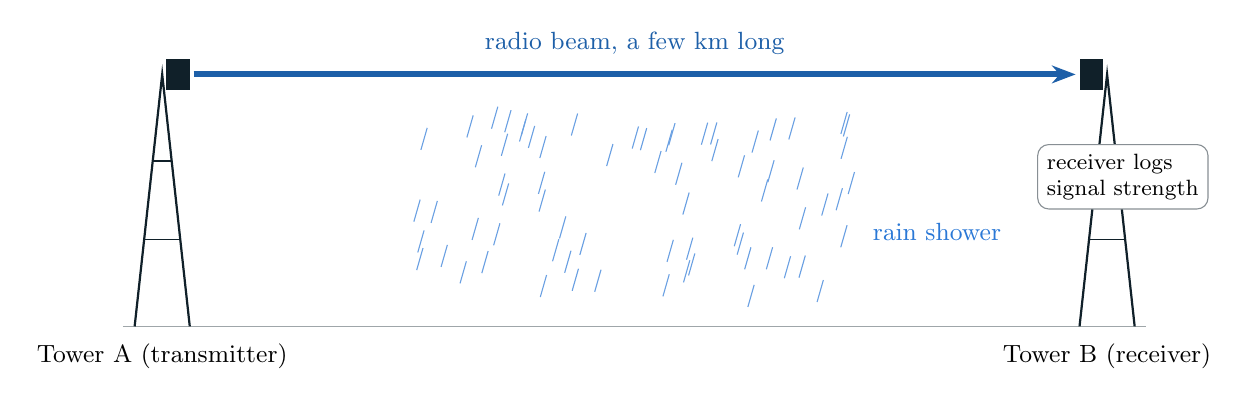
\begin{tikzpicture}[scale=1.0]
  % ground
  \draw[inkc!40] (-0.5,0) -- (12.5,0);
  % towers
  \foreach \x in {0,12} {
    \draw[inkc,thick] (\x-0.35,0) -- (\x,3.2) -- (\x+0.35,0);
    \draw[inkc] (\x-0.22,1.1) -- (\x+0.22,1.1);
    \draw[inkc] (\x-0.12,2.1) -- (\x+0.12,2.1);
  }
  \fill[inkc] (0.05,3.0) rectangle (0.35,3.4);
  \fill[inkc] (11.65,3.0) rectangle (11.95,3.4);
  \node[font=\small,anchor=north] at (0,-0.1) {Tower A (transmitter)};
  \node[font=\small,anchor=north] at (12,-0.1) {Tower B (receiver)};
  % beam
  \draw[beam,line width=2.2pt,-{Stealth[length=3mm]}] (0.4,3.2) -- (11.6,3.2);
  \node[font=\small,beam,anchor=south,fill=white,inner sep=1.5pt] at (6,3.4) {radio beam, a few km long};
  % rain
  \foreach \i in {1,...,70} {
    \pgfmathsetmacro{\rx}{3.2+rnd*5.6}
    \pgfmathsetmacro{\ry}{0.5+rnd*2.3}
    \draw[rainc!70] (\rx,\ry) -- ++(-0.08,-0.28);
  }
  \node[font=\small,anchor=west,rainc] at (8.9,1.2) {rain shower};
  \node[draw=inkc!50,rounded corners,font=\footnotesize,align=left,fill=white] at (12.2,1.9)
     {receiver logs\\ signal strength};
\end{tikzpicture}
\caption{The idea. Tower A sends a radio beam to tower B. Rain between them weakens the beam.
Tower B records how strong the beam arrives. The drop in strength tells us how much it rained
along the path.}
\label{fig:idea}
\end{figure}

Why is this useful? Rain gauges (buckets that measure rain) cover only the spot where they stand,
and Algeria has few of them. Weather radars see wide areas but are expensive and rare. Satellites
see everything but only coarsely: one value per 10\,km square, every 30 minutes. Flash floods,
like Bab El Oued in 2001 or Ghardaïa in 2008, come from short, intense, very local storms that
these tools can miss. Phone networks, on the other hand, already have thousands of links,
densest exactly where people live. Using them costs no new hardware.

\begin{oneline}
Every microwave link between two phone towers is an accidental rain gauge, because rain weakens
the beam, and phone companies already record how strong the beam is.
\end{oneline}

The rest of this document explains each piece in detail: what a radio wave is
(Section~\ref{sec:waves}), how signal strength is measured with decibels (Section~\ref{sec:db}),
how a link works on a dry day (Sections~\ref{sec:network}--\ref{sec:dry}), how rain weakens it
(Section~\ref{sec:rain}), what else can fool us (Section~\ref{sec:fakes}), how we work backwards
from the signal to the rain (Section~\ref{sec:inverse}), and how we check if we got it right
(Section~\ref{sec:scores}).

%==========================================================
\section{Radio waves}
\label{sec:waves}
%==========================================================

\subsection{What a wave is}

Drop a stone in a pond. Ripples spread out: the water goes up and down, and the pattern of ups and
downs travels outwards. That travelling pattern is a \textbf{wave}. The water itself does not travel
far; it just bobs. What travels is the pattern, and with it, energy.

Light is also a wave, but not of water. It is a wave of \emph{electric and magnetic fields}: invisible
forces that push on electric charges. Such a wave is called an \textbf{electromagnetic wave}. It
needs no water or air to travel through; it crosses empty space, which is how sunlight reaches us.

Radio waves are exactly the same kind of thing as light. The only difference is how fast they
wiggle. Our eyes happen to detect waves that wiggle about 500 trillion times per second (we call
them light). Waves that wiggle much more slowly are invisible to us and we call them radio waves.
All electromagnetic waves travel at the \textbf{speed of light}:
\[
c \approx 300\,000\ \text{km per second} = 3\times10^{8}\ \text{metres per second}.
\]
At that speed a radio signal crosses a 5\,km link in about 17 millionths of a second.

\subsection{Frequency and wavelength}

Two numbers describe how a wave wiggles.

\textbf{Frequency} is how many full wiggles (up, down, back to the start) pass a fixed point each
second. Its unit is the \textbf{hertz} (Hz): 1\,Hz means one wiggle per second. Radio frequencies are
huge, so we use bigger units:
\begin{itemize}
  \item 1 kilohertz (kHz) = 1\,000 Hz,
  \item 1 megahertz (MHz) = 1\,000\,000 Hz (FM radio is around 100\,MHz),
  \item 1 gigahertz (GHz) = 1\,000\,000\,000 Hz (Wi-Fi is 2.4 or 5\,GHz).
\end{itemize}
Microwave links between towers use roughly \textbf{6 to 80\,GHz}. In our Swedish data (Gothenburg)
most links use between 28 and 39\,GHz.

\textbf{Wavelength} is the distance from one crest of the wave to the next, written
$\lambda$ (the Greek letter ``lambda''). Frequency and wavelength are tied together by the speed of light:
\begin{equation}
\lambda = \frac{c}{f}
\label{eq:lambda}
\end{equation}
In words: \emph{wavelength equals the speed of light divided by the frequency}. The faster it wiggles,
the shorter the distance between crests.

\begin{figure}[h]
\centering
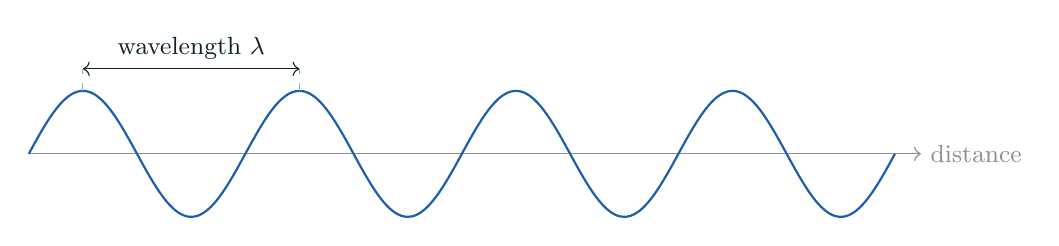
\begin{tikzpicture}[xscale=1.1,yscale=0.8]
  \draw[->,inkc!50] (0,0) -- (10.3,0) node[right,font=\small] {distance};
  \draw[beam,thick,domain=0:10,samples=200,smooth] plot (\x,{sin(\x*180/2.5*2)*1.0});
  \draw[<->,inkc] (0.625,1.35) -- (3.125,1.35) node[midway,above,font=\small] {wavelength $\lambda$};
  \draw[dashed,inkc!40] (0.625,1.0) -- (0.625,1.35);
  \draw[dashed,inkc!40] (3.125,1.0) -- (3.125,1.35);
\end{tikzpicture}
\caption{A wave. The wavelength is the distance between two crests.}
\end{figure}

\begin{example}[: the wavelength of a 38 GHz link]
$f = 38\,\text{GHz} = 38\times10^{9}$ wiggles per second. Then
\[
\lambda = \frac{3\times10^{8}\ \text{m/s}}{38\times10^{9}\ \text{/s}} = 0.0079\ \text{m} \approx 7.9\ \text{mm}.
\]
So the wave crests are about 8 millimetres apart. That is about the size of a large raindrop. This
coincidence matters a lot, as we will see in Section~\ref{sec:rain}.
\end{example}

\begin{table}[h]
\centering\small
\begin{tabular}{rrl}
\toprule
Frequency & Wavelength & Typical use on phone networks \\
\midrule
7 GHz & 43 mm & long links, 20--50 km, in the countryside \\
15 GHz & 20 mm & medium links, 5--20 km \\
23 GHz & 13 mm & links of a few km \\
38 GHz & 7.9 mm & short city links, under 3 km \\
80 GHz & 3.7 mm & very short links, under 1--2 km \\
\bottomrule
\end{tabular}
\caption{Common link frequencies and their wavelengths (from Equation~\ref{eq:lambda}). The
pairing of frequency with link length is typical, not a rule.}
\label{tab:freq}
\end{table}

Why do short links use high frequencies? Because rain and the air weaken high frequencies more (we
will see why), so a high-frequency beam cannot go very far reliably. On the other hand high
frequencies can carry more data and use smaller dishes. So engineers choose a low frequency for long
links and a high one for short links. For us that is good news: short city links are both the most
common and the most sensitive to rain.

\subsection{Polarisation: which way the wave wiggles}

A wave on a rope can wiggle up-and-down or side-to-side. A radio wave can too. The direction in
which its electric field wiggles is called its \textbf{polarisation}. If it wiggles up and down,
the link is \textbf{vertically polarised}; side to side, \textbf{horizontally polarised}. The
transmitting dish decides this. It matters for rain because, as we will see, falling raindrops are
not round: they are flattened, so they are wider than they are tall, and a side-to-side wiggle
``feels'' more water than an up-and-down one.

\subsection{Power}

A transmitter pushes energy into the beam continuously. The amount of energy per second is the
\textbf{power}, measured in \textbf{watts} (W). A microwave link transmitter uses very little: typically
between 0.01\,W and 1\,W, less than a small light bulb. We often use the \textbf{milliwatt}
(mW), one thousandth of a watt.

As the beam travels, its power spreads out and gets absorbed, so the power that reaches the
receiving dish is tiny: often around a millionth of a milliwatt. Numbers this small are awkward,
which is why engineers use decibels.

%==========================================================
\section{Decibels: the language of signal strength}
\label{sec:db}
%==========================================================

This section is the most important tool in the whole document. Take it slowly.

\subsection{The problem decibels solve}

Signal powers span enormous ranges. A transmitter might send 0.1\,W and the receiver might get
0.000\,000\,01\,W. Multiplying and dividing such numbers is clumsy. Decibels turn
\emph{multiplying} into \emph{adding}, and they make huge ranges fit into small numbers.

\subsection{Logarithms, briefly}

The \textbf{logarithm} (base 10) of a number answers the question: \emph{``10 to the power of what
gives this number?''} We write it $\log_{10}$.
\begin{itemize}
  \item $\log_{10}(10) = 1$, because $10^1 = 10$.
  \item $\log_{10}(100) = 2$, because $10^2 = 100$.
  \item $\log_{10}(1000) = 3$.
  \item $\log_{10}(1) = 0$, because $10^0 = 1$.
  \item $\log_{10}(0.01) = -2$, because $10^{-2} = 0.01$.
  \item $\log_{10}(2) \approx 0.301$, because $10^{0.301} \approx 2$.
\end{itemize}
The useful property is that the logarithm of a product is the sum of logarithms:
$\log_{10}(a\times b) = \log_{10}(a) + \log_{10}(b)$. That is how decibels turn multiplication into addition.

\subsection{The decibel}

A \textbf{decibel} (dB) describes the \emph{ratio} between two powers $P_1$ and $P_2$:
\begin{equation}
\text{ratio in dB} = 10 \times \log_{10}\!\left(\frac{P_2}{P_1}\right)
\label{eq:db}
\end{equation}
In words: \emph{divide one power by the other, take the logarithm, multiply by ten}.

\begin{table}[h]
\centering\small
\begin{tabular}{rl}
\toprule
Change in dB & What happens to the power \\
\midrule
$+10$ dB & multiplied by 10 \\
$+3$ dB & roughly doubled \\
$0$ dB & unchanged \\
$-3$ dB & roughly halved \\
$-10$ dB & divided by 10 (90\% lost) \\
$-20$ dB & divided by 100 (99\% lost) \\
$-30$ dB & divided by 1\,000 \\
\bottomrule
\end{tabular}
\caption{Decibels you can do in your head.}
\label{tab:db}
\end{table}

\begin{example}[: what does ``the signal dropped by 9.5 dB'' mean?]
During the storm in our Gothenburg data, the beam on one link arrived 9.5\,dB weaker than on a dry
day. Using Equation~\ref{eq:db} backwards: the power was divided by
$10^{9.5/10} = 10^{0.95} \approx 8.9$. So only about $1/8.9 \approx 11\%$ of the usual power arrived:
rain (and water on the antennas) removed about 89\% of it over a distance of just 1.07\,km.
\end{example}

Because decibels are logarithms, losses \emph{add up}. If the beam loses 3\,dB in one part of the path
and 7\,dB in another, the total loss is 10\,dB, meaning the power was divided by 2 and then by 5,
so by 10 in total. This is why engineers write everything in dB: a whole link becomes a simple
sum of gains and losses.

\subsection{dBm: decibels compared with one milliwatt}

Plain dB describes a \emph{change}. To describe an \emph{amount} of power, we compare it with a fixed
reference of one milliwatt. That unit is the \textbf{dBm}:
\begin{equation}
P \text{ in dBm} = 10 \times \log_{10}\!\left(\frac{P}{1\ \text{mW}}\right)
\end{equation}

\begin{table}[h]
\centering\small
\begin{tabular}{rl}
\toprule
Power in dBm & Power in milliwatts \\
\midrule
$+20$ dBm & 100 mW \\
$+10$ dBm & 10 mW (a typical transmitter in our Swedish data) \\
$0$ dBm & 1 mW \\
$-30$ dBm & 0.001 mW \\
$-45$ dBm & 0.000\,03 mW (a typical received signal in our data) \\
$-60$ dBm & 0.000\,001 mW \\
$-80$ dBm & 0.000\,000\,01 mW (near the limit: the link starts to fail) \\
\bottomrule
\end{tabular}
\caption{dBm values. Negative dBm means less than one milliwatt. Every $-10$\,dBm step divides the power by 10.}
\end{table}

Phone companies record two numbers for every link:
\begin{itemize}
\item the \textbf{transmitted signal level} (TSL): how much power the sending dish puts out, in dBm;
\item the \textbf{received signal level} (RSL): how much power arrives at the receiving dish, in dBm.
\end{itemize}
The difference between them, TSL $-$ RSL, is the \textbf{total loss} of the link in dB. Everything in
this project starts from that difference.

%==========================================================
\section{How a phone network uses microwave links}
\label{sec:network}
%==========================================================

\subsection{Two kinds of connection}

When you make a call, your phone talks by radio to the nearest tower. That is the
\textbf{access} part of the network, and it is not what we use. The tower then has to pass your data
on, towards the operator's central computers and the internet. That tower-to-tower and
tower-to-centre part is called \textbf{backhaul}. Backhaul uses either buried fibre-optic cables or
microwave links. Microwave links are cheaper and faster to install, so they are very common,
especially in growing cities and rural areas.

\subsection{What a link looks like}

A microwave link is a pair of dish antennas, usually 20\,cm to 1\,m across, mounted high on two
towers or rooftops and pointed exactly at each other. The dishes are usually covered by a flat
plastic or fabric lid called a \textbf{radome} that keeps rain and birds out. (Remember the
radome; it will cause trouble in Section~\ref{sec:fakes}.)

The two dishes must \textbf{see each other}: there must be a clear, straight line between them with no
building or hill in the way. Engineers call this \textbf{line of sight}.

Most links talk in \textbf{both directions} at once, using two slightly different frequencies. So one
physical link gives us two separate measurements: A$\to$B and B$\to$A. In our data each direction is
called a \textbf{sub-link}. Gothenburg's network has 364 links, so 728 sub-links. Their lengths range
from 0.14\,km to 15\,km, with a typical (median) length of 2.3\,km.

\subsection{What the operator records}

The operator's \textbf{network management system} (a central computer program that watches every
piece of equipment) asks each radio, regularly, for its current transmitted and received levels.
How often depends on the operator:
\begin{itemize}
\item In our Swedish data, one reading every \textbf{10 seconds}.
\item In our Italian data, one reading every \textbf{minute}.
\item In our Dutch data, the system keeps only the \textbf{lowest and highest} received level in each
\textbf{15-minute} window. This is the most common format operators can export, and the hardest one
for us.
\end{itemize}
The readings are rounded. Some radios report in steps of 0.1\,dB, others only in whole decibels
(steps of 1\,dB). This rounding is called \textbf{quantisation}, and it limits how little rain we
can notice (Section~\ref{sec:inverse}).

%==========================================================
\section{A link on a dry day}
\label{sec:dry}
%==========================================================

Even without rain, the received power is far smaller than the transmitted power. Engineers add up
every gain and loss along the way in a \textbf{link budget}. Because everything is in decibels, the
budget is a simple sum.

\subsection{Spreading: the free-space loss}

Even a narrow beam spreads out like the light from a torch. The further it travels, the larger the
area it covers, so the less of it lands on the receiving dish. This loss happens even in perfectly
empty space, so it is called \textbf{free-space path loss}. A standard formula gives it in dB:
\begin{equation}
L_\text{free} = 20\log_{10}(d) + 20\log_{10}(f) + 92.45
\label{eq:fspl}
\end{equation}
where $d$ is the distance in kilometres and $f$ the frequency in GHz. In words: \emph{the loss grows with
distance and with frequency}. Doubling the distance adds $20\log_{10}(2) \approx 6$\,dB of loss.

\begin{example}[: free-space loss of a 1 km link at 38 GHz]
$L_\text{free} = 20\log_{10}(1) + 20\log_{10}(38) + 92.45 = 0 + 31.6 + 92.45 \approx 124$\,dB.
That means the power is divided by $10^{12.4}$, about 2.5 trillion. It sounds hopeless, but the dishes
fix most of it.
\end{example}

\subsection{Focusing: the antenna gain}

A dish does not spray power in all directions; it focuses it into a narrow beam, like a torch
compared with a bare bulb. Compared with spraying evenly in all directions, a dish delivers far more
power in its pointing direction. This advantage is the \textbf{antenna gain}, in dB. A typical dish of
30--60\,cm at these frequencies has a gain of roughly 35--45\,dB. The receiving dish has a gain too,
because it collects power over its whole surface.

\subsection{The budget}

\begin{equation}
\text{RSL} = \text{TSL} + G_\text{transmit} + G_\text{receive} - L_\text{free} - L_\text{other}
\label{eq:budget}
\end{equation}
In words: \emph{the received level equals the transmitted level, plus the boost from both dishes,
minus the spreading loss and any other losses}. ``Other losses'' include cables and connectors, and,
importantly for us, rain.

\begin{figure}[h]
\centering
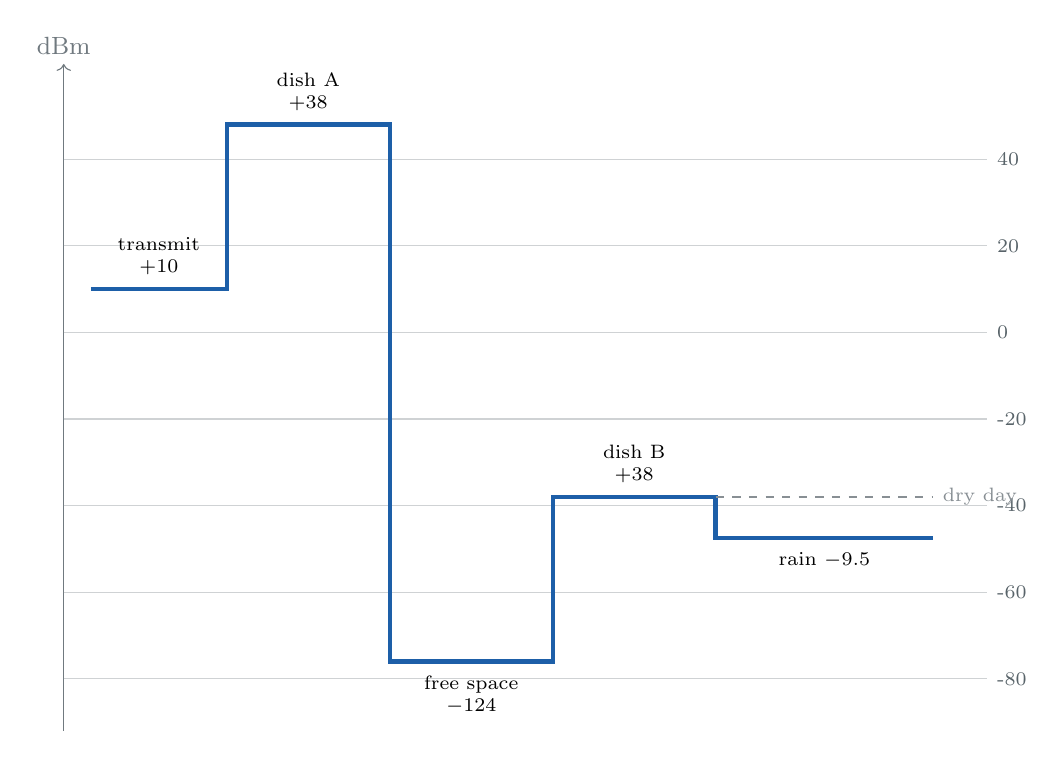
\begin{tikzpicture}[yscale=0.055,xscale=1.15]
  \draw[->,inkc!60] (0,-92) -- (0,62) node[above,font=\small] {dBm};
  \foreach \y in {-80,-60,-40,-20,0,20,40} \draw[inkc!20] (0,\y) -- (10.2,\y) node[right,font=\scriptsize,inkc!70]{\y};
  \draw[beam,line width=1.6pt] (0.3,10) -- (1.8,10) -- (1.8,48) -- (3.6,48) -- (3.6,-76) -- (5.4,-76) -- (5.4,-38) -- (7.2,-38) -- (7.2,-47.5) -- (9.6,-47.5);
  \node[font=\scriptsize,align=center,anchor=south] at (1.05,11) {transmit\\$+10$};
  \node[font=\scriptsize,align=center,anchor=south] at (2.7,49) {dish A\\$+38$};
  \node[font=\scriptsize,align=center,anchor=north] at (4.5,-77) {free space\\$-124$};
  \node[font=\scriptsize,align=center,anchor=south] at (6.3,-37) {dish B\\$+38$};
  \node[font=\scriptsize,align=center,anchor=north] at (8.4,-48.5) {rain $-9.5$};
  \draw[dashed,inkc!50] (7.2,-38) -- (9.6,-38) node[right,font=\scriptsize]{dry day};
\end{tikzpicture}
\caption{A link budget as a staircase (illustrative values for a 1\,km, 38\,GHz link). The signal
starts at the transmitter, is boosted by dish A, loses 124\,dB crossing 1\,km of space, is boosted by
dish B, and arrives around $-38$\,dBm on a dry day. In a storm, rain removes several more dB.}
\end{figure}

\subsection{The beam is fatter than a line}

The beam is not an infinitely thin line. Radio energy travels through a cigar-shaped region around
the straight line between the dishes. Physicists call it the \textbf{Fresnel zone} (pronounced
``freh-nel''). Its radius in the middle of the link is about
\begin{equation}
r \approx 17.32\sqrt{\frac{d}{4f}} \ \text{metres}
\end{equation}
with $d$ in km and $f$ in GHz. For a 1\,km link at 38\,GHz, $r \approx 1.4$\,m; for a 10\,km link at
15\,GHz, $r \approx 7$\,m. So a link ``sees'' the rain inside a long, thin tube, a few metres wide, between
the two dishes.

\subsection{The dry-day signal is not perfectly steady}

Even with no rain, the received level wobbles a little:
\begin{itemize}
\item \textbf{Water vapour and oxygen} in the air absorb a little energy. This changes slowly with
humidity and temperature, and amounts to a fraction of a dB per km.
\item \textbf{Temperature} affects the electronics slightly, causing slow daily ups and downs.
\item On long links, layers of warm and cool air can bend the beam, or make part of it bounce off
the ground or water and arrive slightly late, partly cancelling the main beam. This is called
\textbf{multipath fading} and can cause sudden dips, especially at night.
\item Some links automatically turn up their transmit power when the signal gets weak. This is called
\textbf{automatic transmit power control}. It is why we need the transmitted level as well as the received one: if
TSL goes up by 5\,dB and RSL stays the same, the path loss actually grew by 5\,dB.
\end{itemize}
The normal dry-weather level of TSL $-$ RSL is called the \textbf{baseline}. Rain shows up as loss
\emph{above} the baseline.

%==========================================================
\section{How rain weakens the beam}
\label{sec:rain}
%==========================================================

\subsection{What a raindrop is like}

Raindrops range from about 0.1\,mm (drizzle) to about 6\,mm across; bigger ones break apart while falling.
Small drops are round. Large drops are not tear-shaped, as cartoons show: air pushes up on their
bottom as they fall, so they flatten into a shape like a hamburger bun, wider than tall.

\begin{figure}[h]
\centering
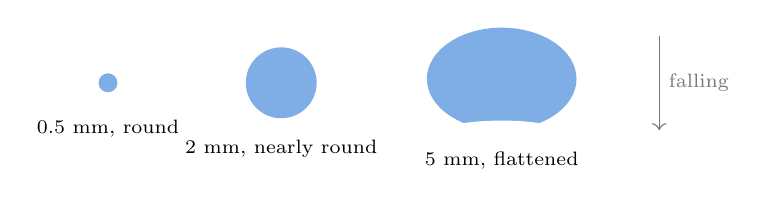
\begin{tikzpicture}
  \fill[rainc!60] (0,0) circle (0.12);
  \node[font=\scriptsize,below] at (0,-0.35) {0.5 mm, round};
  \fill[rainc!60] (2.2,0) circle (0.45);
  \node[font=\scriptsize,below] at (2.2,-0.6) {2 mm, nearly round};
  \fill[rainc!60] (5,0.05) ellipse (0.95 and 0.65);
  \fill[white] (5,-0.6) ellipse (0.7 and 0.12);
  \node[font=\scriptsize,below] at (5,-0.75) {5 mm, flattened};
  \draw[->,inkc!60] (7.0,0.6) -- (7.0,-0.6) node[midway,right,font=\scriptsize]{falling};
\end{tikzpicture}
\caption{Raindrop shapes (not to scale with each other). Large drops are flattened by the air they fall through.}
\end{figure}

How much rain is falling is measured as a \textbf{rain rate}, in \textbf{millimetres per hour}
(mm/h): if the rain kept falling at this intensity for one hour and none of it drained away, it
would form a layer this many millimetres deep. As a rough feel:
\begin{center}\small
\begin{tabular}{rl}
\toprule
Rain rate & What it feels like \\
\midrule
0.1--1 mm/h & drizzle, light rain \\
around 5 mm/h & moderate rain, umbrella needed \\
around 20 mm/h & heavy downpour, streets start to stream \\
50--100+ mm/h & violent rain, typical of flash-flood storms (for minutes, not hours) \\
\bottomrule
\end{tabular}
\end{center}

\subsection{Two ways a drop takes energy from the beam}

When the radio wave passes a raindrop, its electric field pushes the water molecules back and forth
(water molecules are slightly charged at each end, so they respond strongly to electric fields).
This does two things:
\begin{enumerate}
\item \textbf{Absorption.} The jostled molecules turn some of the wave's energy into heat, warming the drop
by an immeasurably tiny amount. This is the same physics as a microwave oven, at a far lower power.
\item \textbf{Scattering.} The drop re-radiates part of the energy in other directions, like a tiny
antenna of its own. That energy leaves the beam and never reaches the receiver.
\end{enumerate}
Both remove power from the beam. Together they are called \textbf{attenuation}: the weakening of the
signal, measured in dB.

\subsection{Why frequency matters so much}

A drop affects the wave most strongly when its size is comparable to the wavelength. At 7\,GHz the
wavelength (43\,mm) is far bigger than any raindrop, and the drops barely disturb it. At 38\,GHz the
wavelength (8\,mm) is comparable to big drops, and the effect is strong. That is why short city
links at high frequencies are the most useful rain sensors, and why long rural links at low
frequencies only notice heavy rain.

\subsection{The power law: from rain rate to loss per kilometre}

Scientists and engineers have measured and calculated how much loss rain causes at each frequency.
The international reference is a recommendation from the International Telecommunication Union
(ITU), a United Nations agency that sets radio standards. It is called \textbf{ITU-R P.838}
(version 3, 2005). It says that the loss per kilometre of rain follows a simple formula:
\begin{equation}
k = a \, R^{\,b}
\label{eq:kR}
\end{equation}
where
\begin{itemize}
\item $R$ is the rain rate in mm/h,
\item $k$ is the \textbf{specific attenuation}: the loss in dB for each kilometre of rainy path,
\item $a$ and $b$ are two numbers that depend on the frequency and polarisation, published in tables by the ITU.
\end{itemize}
In words: \emph{the loss per kilometre equals a frequency-dependent number $a$, times the rain rate raised to
a frequency-dependent power $b$}. ``Raised to the power $b$'' means: if $b=1$, then $R^b = R$ and the loss is
simply proportional to the rain (twice the rain, twice the loss). If $b$ is bigger than 1, the loss grows
faster than the rain; if smaller, slower.

\begin{table}[h]
\centering\small
\begin{tabular}{rcccc}
\toprule
& \multicolumn{2}{c}{Vertical polarisation} & \multicolumn{2}{c}{Horizontal polarisation} \\
\cmidrule(lr){2-3}\cmidrule(lr){4-5}
Frequency & $a$ & $b$ & $a$ & $b$ \\
\midrule
7 GHz  & 0.00142 & 1.475 & 0.00192 & 1.481 \\
15 GHz & 0.0501 & 1.044 & 0.0448 & 1.123 \\
23 GHz & 0.128 & 0.963 & 0.129 & 1.021 \\
38 GHz & 0.384 & 0.855 & 0.400 & 0.882 \\
80 GHz & 1.167 & 0.702 & 1.170 & 0.712 \\
\bottomrule
\end{tabular}
\caption{ITU-R P.838-3 coefficients, as computed by the open-source pycomlink library we use.}
\label{tab:ab}
\end{table}

\begin{example}[: how much does 20 mm/h of rain weaken a 38 GHz beam?]
For 38\,GHz, vertical: $a = 0.384$, $b = 0.855$. With $R = 20$\,mm/h:
\[
k = 0.384 \times 20^{0.855}.
\]
First $20^{0.855}$: that is $10^{0.855\times\log_{10}20} = 10^{0.855\times1.301} = 10^{1.112} \approx 12.9$.
So $k \approx 0.384\times12.9 \approx 5.0$\,dB per km. Over a 1\,km link that is 5\,dB: the received power
drops to about a third. At 7\,GHz the same rain gives only $0.00142\times20^{1.475}\approx0.12$\,dB per km,
forty times less.
\end{example}

\begin{figure}[h]
\centering
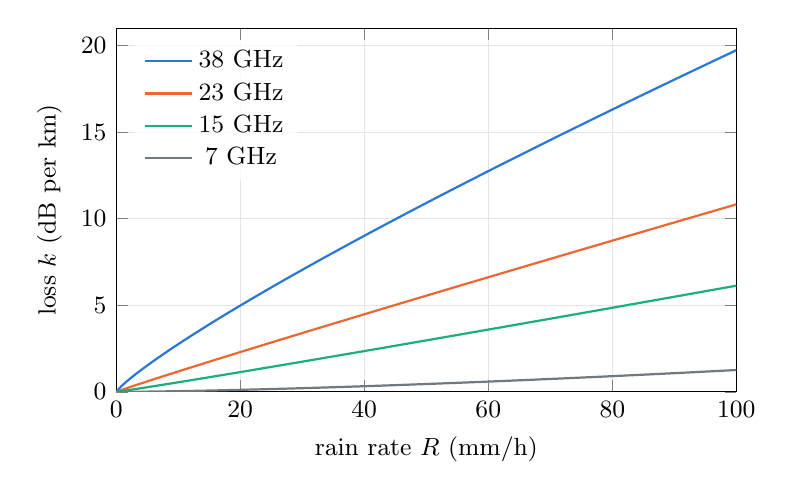
\begin{tikzpicture}
\begin{axis}[width=0.78\textwidth,height=6.2cm,xlabel={rain rate $R$ (mm/h)},ylabel={loss $k$ (dB per km)},
  xmin=0,xmax=100,ymin=0,ymax=21,grid=major,grid style={inkc!12},legend pos=north west,
  legend style={font=\small,draw=none,fill=white,fill opacity=0.8,text opacity=1},tick label style={font=\small},label style={font=\small}]
  \addplot[domain=0:100,samples=120,thick,color=rainc] {0.3844*x^0.8552}; \addlegendentry{38 GHz}
  \addplot[domain=0:100,samples=120,thick,color=gaugec] {0.1284*x^0.963}; \addlegendentry{23 GHz}
  \addplot[domain=0:100,samples=120,thick,color=radarc] {0.05008*x^1.044}; \addlegendentry{15 GHz}
  \addplot[domain=0:100,samples=120,thick,color=inkc!60] {0.00142*x^1.4745}; \addlegendentry{7 GHz}
\end{axis}
\end{tikzpicture}
\caption{Loss per kilometre against rain rate for four frequencies (vertical polarisation,
Equation~\ref{eq:kR}). Higher frequencies are far more sensitive. Around 20--30\,GHz the curves are
almost straight lines ($b \approx 1$), which makes the measurement especially convenient.}
\label{fig:kR}
\end{figure}

Notice in Table~\ref{tab:ab} that horizontal polarisation has slightly larger $a$ or $b$ than vertical.
That is the flattened drops at work: a side-to-side wiggle travels through more water.

\subsection{From loss per kilometre to the whole link}

Rain is rarely the same along the whole link. The total rain loss is the sum of the losses on each
little piece of the path. If we split the link into many short pieces, each of length $\Delta x$ with
its own rain rate, then
\begin{equation}
A = \sum_\text{pieces} k(\text{rain on that piece}) \times \Delta x
\end{equation}
($A$ for attenuation, in dB). With infinitely small pieces, mathematicians write this sum as an integral,
$A = \int_0^L k(x)\,dx$, which means the same thing: add up loss per km times km, all along the path of
length $L$.

If the rain is the same everywhere along the link, this becomes simply
\begin{equation}
A = k \times L = a R^{\,b} L
\label{eq:A}
\end{equation}
In practice we use Equation~\ref{eq:A} and interpret the $R$ we get as a kind of \textbf{average rain along the
link}. Each link therefore measures a \emph{line} of rain, not a point like a gauge. For links of a few km,
that is exactly the scale at which flash floods start in a city.

%==========================================================
\section{Things that look like rain but are not}
\label{sec:fakes}
%==========================================================

A drop in signal does not always mean rain in the air. These are the main impostors.

\subsection{The wet antenna}

When it rains, water also lands on the radomes, the plastic lids over the dishes. A thin film of
water sits right in front of the antenna, and the beam must pass through it. That film weakens the
signal too, sometimes by several dB, and it has nothing to do with how much rain falls between the
towers. This is called \textbf{wet antenna attenuation}.

It is large. In our worked example (Section~\ref{sec:inverse}), the model we use estimates that 4.1 of the
9.5\,dB lost at the peak of the storm came from wet antennas, not from rain in the air. Without correcting for it,
our links reported 3.5 times too much rain over June and July 2015. Different correction methods exist; we tested
several and chose the one that matched the rain gauges best during our tuning months.

The film also lingers after the rain stops, while the radome dries, so the signal recovers slowly.

\subsection{Other impostors}
\begin{itemize}
\item \textbf{Wet snow and melting snow} weaken the beam much more than rain for the same amount of water.
In Algeria's coastal cities this is rare.
\item \textbf{Dew and fog} can wet the radomes without any rain.
\item \textbf{Multipath fading} (Section~\ref{sec:dry}) causes sudden dips on long links, often at night.
\item \textbf{Equipment changes}: a technician re-aligns a dish or replaces a radio, and the baseline jumps.
\item \textbf{Dust and sand}. Dry dust weakens these beams much less than rain does, but there is almost no
published data from real phone links during sand storms. For Algeria this is an open question. We say so
honestly and plan to model it as an uncertain extra term in our simulation.
\item \textbf{Faulty links}. Some links in our data report wild swings all the time. Our quality check removed
45 of the 728 Swedish sub-links because they claimed rain more than 30\% of the time, when the radar showed it
never rained on any path more than 9.4\% of the time.
\end{itemize}

%==========================================================
\section{Working backwards: from the signal to the rain}
\label{sec:inverse}
%==========================================================

Now we put everything together. This is the classical method (no AI) that our project reproduced as
its baseline. We follow one real link through one real storm.

\begin{center}\small
Link: sub-link 718, Gothenburg. Length $L = 1.07$\,km. Frequency $f = 37.32$\,GHz, vertical polarisation.\\
A rain gauge stands 4\,m from the beam's path. Date: 25 August 2015.
\end{center}

\begin{figure}[h]
\centering
\begin{tikzpicture}
\begin{groupplot}[group style={group size=1 by 2,vertical sep=0.9cm,xlabels at=edge bottom},
  width=0.95\textwidth,height=4.8cm,xmin=4,xmax=24,xtick={4,6,...,24},grid=major,grid style={inkc!12},
  tick label style={font=\small},label style={font=\small},legend style={font=\scriptsize,draw=none,fill=white,fill opacity=0.85,text opacity=1}]
\nextgroupplot[ylabel={total loss (dB)},ymin=47.5,ymax=59,legend pos=north east]
  \addplot[very thin,color=rainc,forget plot] table[x=hour,y=tl] {storm.dat};
  \addplot[thick,dashed,color=inkc!60,forget plot] table[x=hour,y=base] {storm.dat};
  \addlegendimage{thick,color=rainc} \addlegendentry{total loss, TSL $-$ RSL}
  \addlegendimage{thick,dashed,color=inkc!60} \addlegendentry{dry-weather baseline}
\nextgroupplot[ylabel={rain (mm/h)},xlabel={hour of the day (UTC), 25 August 2015},ymin=0,ymax=24,legend pos=north east]
  \addplot[thick,color=gaugec,forget plot] table[x=hour,y=gauge] {storm.dat};
  \addplot[thick,color=rainc,forget plot] table[x=hour,y=R] {storm.dat};
  \addplot[only marks,mark=*,mark size=1.2pt,color=radarc,forget plot] table[x=hour,y=R] {radar.dat};
  \addlegendimage{thick,color=gaugec} \addlegendentry{rain gauge (5-min average)}
  \addlegendimage{thick,color=rainc} \addlegendentry{link estimate (5-min average)}
  \addlegendimage{only marks,mark=*,mark size=1.6pt,color=radarc} \addlegendentry{weather radar}
\end{groupplot}
\end{tikzpicture}
\caption{Real data. Top: the total loss of the link through the day, and the dry-weather baseline the
method estimated. Bottom: the rain worked out from the link, compared with the rain gauge next to it and with
the weather radar. Times before 04:00 were dry and are cut off.}
\label{fig:storm}
\end{figure}

\subsection*{Step 1: total loss}
For every minute, compute TSL $-$ RSL in dB. On this link it sits around 48.7\,dB on a dry day, and climbs to
58.2\,dB at 08:30, the peak of the storm (Figure~\ref{fig:storm}, top).

\subsection*{Step 2: is it raining?}
Rain does not just lower the signal; it makes it \emph{jumpy}, because rain cells come and go. Dry-day signals are
calm. So we measure how jumpy the signal is with the \textbf{standard deviation}: a number that says how far, on
average, values stray from their own average. For each minute we take the 60 minutes centred on it, compute
their standard deviation, and call the minute \textbf{wet} if it is above a threshold. We tried thresholds from 0.1
to 1.5\,dB and window lengths of 15, 30 and 60 minutes on June and July data, and kept the best: \textbf{60
minutes and 0.35\,dB}.

One honest weakness: a window centred on the current minute uses the next 30 minutes too. For a live warning
system that is too late. The AI models in the next phase will only look at the past.

\subsection*{Step 3: the baseline}
When a wet period starts, we freeze the baseline at the average of the last 5 dry minutes before it, and hold
it until the rain ends. Any loss above the baseline counts as caused by rain. At 08:30 the baseline was 48.71\,dB, so
\[
A_\text{observed} = 58.18 - 48.71 = 9.47\ \text{dB}.
\]

\subsection*{Step 4: remove the wet antenna}
The wet-antenna model we use (from Pastorek and colleagues, as implemented in pycomlink) estimates
4.10\,dB of antenna loss here, leaving
\[
A_\text{rain} = 9.47 - 4.10 = 5.37\ \text{dB}
\]
caused by rain in the air.

\subsection*{Step 5: turn loss into rain}
Solve Equation~\ref{eq:A} for $R$. Dividing both sides by $aL$ and taking the $b$-th root:
\begin{equation}
R = \left(\frac{A}{a\,L}\right)^{1/b}
\label{eq:inverse}
\end{equation}
In words: \emph{loss divided by (coefficient times length), raised to the power one-over-$b$}.

\begin{example}[: the rain at 08:30]
At 37.32\,GHz vertical, the ITU coefficients are $a = 0.370$ and $b = 0.860$. Then
\[
\frac{A}{aL} = \frac{5.37}{0.370\times1.07} = 13.6, \qquad
R = 13.6^{1/0.860} = 13.6^{1.163} \approx 20.7\ \text{mm/h}.
\]
Without the wet-antenna correction we would have used $A = 9.47$ and obtained about 40\,mm/h, twice as much.
Averaged over the 5 minutes around 08:30, the link says 17.3\,mm/h and the gauge says 14.4\,mm/h.
\end{example}

\subsection*{How little rain can a link notice?}
Because readings are rounded (quantisation), the smallest change a link can report is 0.1\,dB or 1\,dB. Using
Equation~\ref{eq:inverse}, here is how much rain that smallest step represents:
\begin{center}\small
\begin{tabular}{lcc}
\toprule
Link & rain equal to a 0.1 dB step & rain equal to a 1 dB step \\
\midrule
38 GHz, 1 km & 0.2 mm/h & 3.1 mm/h \\
23 GHz, 3 km & 0.25 mm/h & 2.7 mm/h \\
15 GHz, 8 km & 0.26 mm/h & 2.4 mm/h \\
7 GHz, 20 km & 2.3 mm/h & 11 mm/h \\
\bottomrule
\end{tabular}
\end{center}
So a well-chosen link with fine rounding notices light rain, while a long low-frequency link with coarse rounding
only notices heavy rain. For flash floods, heavy rain is exactly what matters.

%==========================================================
\section{How we check if we got it right}
\label{sec:scores}
%==========================================================

To judge the method, we compare it with two references. \textbf{Rain gauges} measure rain directly but only at one
spot. The \textbf{weather radar} sees the whole area but estimates rain indirectly from echoes, so it has errors of
its own. Neither is perfect, so we use both.

We tuned everything on June and July 2015 and tested once on August 2015, a month the method had never seen. This
separation matters: testing on the tuning data would make any method look better than it really is.

\subsection{Rain or no rain}
For each 5-minute period we compare the method's ``wet/dry'' with the radar's. Four outcomes are possible:
\begin{center}\small
\begin{tabular}{lcc}
\toprule
& radar says rain & radar says dry \\
\midrule
method says rain & correct alarm (TP) & false alarm (FP) \\
method says dry & miss (FN) & correct quiet (TN) \\
\bottomrule
\end{tabular}
\end{center}
From these counts:
\begin{itemize}
\item \textbf{True positive rate} $=\text{TP}/(\text{TP}+\text{FN})$: of the rainy periods, what share did we catch? Ours: \textbf{71\%}.
\item \textbf{False positive rate} $=\text{FP}/(\text{FP}+\text{TN})$: of the dry periods, what share did we wrongly call rainy? Ours: \textbf{4.6\%}.
\item \textbf{Matthews correlation coefficient} (MCC) summarises both in one number:
\[
\text{MCC} = \frac{\text{TP}\cdot\text{TN} - \text{FP}\cdot\text{FN}}
{\sqrt{(\text{TP}+\text{FP})(\text{TP}+\text{FN})(\text{TN}+\text{FP})(\text{TN}+\text{FN})}}
\]
It is 1 for a perfect detector, 0 for random guessing. It is fairer than ``percent correct'' when, as here,
dry periods vastly outnumber rainy ones (a detector that always says ``dry'' would be 90\% correct but useless).
Ours: \textbf{0.58}.
\end{itemize}

\subsection{How much rain}
For amounts we compare hourly rain from links with hourly rain from the gauges near them:
\begin{itemize}
\item \textbf{Correlation} $r$: do the two go up and down together? 1 means perfectly in step, 0 means no relation.
Ours: \textbf{0.81}. For comparison, the weather radar against the same gauges: 0.80.
\item \textbf{Root mean square error} (RMSE): the typical size of a mistake, in mm/h. Square every error, average them,
take the square root. Squaring makes large mistakes count more. Ours: \textbf{1.04\,mm/h}.
\item \textbf{Bias}: does the method measure too much or too little overall, as a percentage of the total? Ours: \textbf{$-6\%$}
(slightly too little).
\end{itemize}

In short, on a month it had never seen, the classical method measured hourly rain about as well as the weather radar,
using only equipment that already exists. Its weaknesses are noisy 5-minute values, the need to look 30 minutes into
the future, and two settings tuned by hand. Those are what the AI is meant to improve.

%==========================================================
\section{Where AI comes in, and what comes after}
%==========================================================

The steps in Section~\ref{sec:inverse} are fixed rules chosen by people. Two of them are the weakest: deciding whether it
rains (Step~2) and turning the signal into rain while accounting for wet antennas and noise (Steps~4--5). A
\textbf{neural network} is a program that learns such rules from examples instead of being told them. We will show it
months of signal recordings together with what the radar and gauges measured at the same time, and let it learn the
patterns, including subtle ones a human would not write down (for example, the shape of a wet antenna drying). We will
use small networks that look only at the past, so they can run live. The test is the same August month, and the bar to
beat is the set of numbers above.

Then:
\begin{itemize}
\item \textbf{Rain maps.} Hundreds of links crossing a city each give a line-average of rain. Combining them gives a map
of rain over the whole city every few minutes. Pushing that map forward in the direction the storm moves gives a forecast
for the next 30--60 minutes.
\item \textbf{Flood risk.} Rain only floods a street if the water collects there. Combining the rain map with the shape of the
land (valleys, dry riverbeds called \emph{wadis}, slopes) and with how much ground is covered by concrete and asphalt tells us
which neighbourhoods and roads are most at risk in the next hour.
\item \textbf{Algeria.} Real link records from Algerian operators are not public. We know where Algerian towers are (from
OpenCelliD, a public map built from phones that report which tower they see and where they are), but not which towers are
joined by microwave links, nor their signal records. So for Algeria we will build \emph{simulated} links between real tower
positions, and feed them real storms measured by NASA satellites. That demonstrates the system; it does not prove its accuracy
there. Proving it needs a pilot with an operator and the national weather service.
\end{itemize}

%==========================================================
% PART 2: the AI model (Phase 2). Added after Phase 2 was run.
% Everything before this point is unchanged.
%==========================================================
% generated by scripts/export_explainer_varied.py -- do not edit
\newcommand{\SeedRows}{0 & $-$12\% & 0.87 & $-$28\% & 0.69 & 10\% / 10\%\\
1 & $+$7\% & 1.01 & $-$14\% & 0.79 & 12\% / 16\%\\
2 & $+$16\% & 1.12 & $-$5\% & 0.89 & 11\% / 16\%\\
3 & $+$6\% & 1.02 & $-$18\% & 0.77 & 11\% / 14\%\\
4 & $+$5\% & 1.02 & $-$14\% & 0.81 & 12\% / 15\%\\}
\newcommand{\SeedValTestR}{0.97}
\newcommand{\ExpRows}{Sweden only (as before) & 0.62 & $-$32\% to $-$6\% & $-$6\% to $+$41\% & 83\% & 32\%\\
Sweden only, rate error in log scale & 0.62 & $-$20\% to $+$9\% & $-$8\% to $+$32\% & 81\% & 48\%\\
Sweden + Italy 2021 & 0.65 & $-$17\% to $+$0\% & $-$3\% to $+$4\% & 95\% & 28\%\\
Sweden + Italy 2021, log scale & 0.65 & $-$23\% to $-$16\% & $-$15\% to $-$5\% & 83\% & 20\%\\
Sweden + Italy 2021 + neighbour inputs & 0.68 & $-$17\% to $-$11\% & $-$16\% to $+$0\% & 91\% & 35\%\\
Sweden + Italy 2021, reliable links only & 0.65 & $-$18\% to $-$13\% & $-$7\% to $+$5\% & 95\% & 42\%\\
\quad + hidden + rate error on 15-minute averages (not kept) & 0.65 & $-$24\% to $-$13\% & $-$8\% to $-$2\% & 91\% & 50\%\\
\quad + Swedish radar corrected with gauges & 0.65 & $-$13\% to $-$9\% & $-$4\% to $+$12\% & 94\% & 40\%\\
\quad + unclear moments hidden & 0.65 & $-$15\% to $-$11\% & $-$5\% to $+$5\% & 93\% & 56\%\\
\quad + both of the above & 0.65 & $-$13\% to $-$6\% & $+$1\% to $+$11\% & 95\% & 55\%\\
\quad + hidden + gauge answers in Italy & 0.65 & $-$15\% to $+$2\% & $+$5\% to $+$11\% & 97\% & 67\%\\
\textbf{\quad + all three (final recipe)} & 0.65 & $-$11\% to $+$1\% & $+$5\% to $+$13\% & 96\% & 66\%\\
\quad + shorter memory (not kept) & 0.66 & $-$14\% to $-$4\% & $-$2\% to $+$5\% & 95\% & 51\%\\
\quad + corrected + hidden + shorter memory (not kept) & 0.65 & $-$8\% to $-$3\% & $-$2\% to $+$8\% & 93\% & 59\%\\}
\newcommand{\ExpRelSeRange}{$-$18\% and $-$13\%}
\newcommand{\ExpRelLong}{42\%}
\newcommand{\ExpFinSeRange}{$-$11\% and $+$1\%}
\newcommand{\ExpFinLong}{66\%}
\newcommand{\NlRelWestLong}{66\%}
\newcommand{\NlRelWestGauges}{91\%}
\newcommand{\NlRelEastLong}{22\%}
\newcommand{\NlRelEastGauges}{84\%}
\newcommand{\NlFinWestLong}{93\%}
\newcommand{\NlFinWestGauges}{93\%}
\newcommand{\NlFinEastLong}{30\%}
\newcommand{\NlFinEastGauges}{87\%}
\newcommand{\NlRows}{reliable links only & west $\to$ east & $+$4\% to $+$19\% & 91\% & 104\% & 66\%\\
reliable links only & east $\to$ west & $-$13\% to $-$12\% & 84\% & 84\% & 22\%\\
\textbf{final recipe} & west $\to$ east & $+$9\% to $+$37\% & 93\% & 103\% & 93\%\\
\textbf{final recipe} & east $\to$ west & $-$13\% to $-$6\% & 87\% & 82\% & 30\%\\}
\newcommand{\CVallSeMCC}{0.651}
\newcommand{\CVallSeR}{0.83}
\newcommand{\CVallSeRMSE}{0.97}
\newcommand{\CVallSeBias}{$-$14\%}
\newcommand{\CVallSeBiasRange}{$-$19\% to $-$6\%}
\newcommand{\CVallBiasA}{$+$3\% to $+$15\%}
\newcommand{\CVallLongAa}{94\%}
\newcommand{\CVallLongAb}{94\%}
\newcommand{\CVallLongAc}{86\%}
\newcommand{\CVallLongAd}{96\%}
\newcommand{\CVallGaugesA}{88\%}
\newcommand{\CVallBiasB}{$-$1\% to $+$8\%}
\newcommand{\CVallLongBa}{99\%}
\newcommand{\CVallLongBb}{102\%}
\newcommand{\CVallLongBc}{86\%}
\newcommand{\CVallLongBd}{50\%}
\newcommand{\CVallGaugesB}{84\%}
\newcommand{\CVrelSeMCC}{0.648}
\newcommand{\CVrelSeR}{0.81}
\newcommand{\CVrelSeRMSE}{1.01}
\newcommand{\CVrelSeBias}{$-$17\%}
\newcommand{\CVrelSeBiasRange}{$-$23\% to $-$12\%}
\newcommand{\CVrelBiasA}{$+$1\% to $+$4\%}
\newcommand{\CVrelLongAa}{93\%}
\newcommand{\CVrelLongAb}{94\%}
\newcommand{\CVrelLongAc}{87\%}
\newcommand{\CVrelLongAd}{95\%}
\newcommand{\SeOnlyLongAa}{77\%}
\newcommand{\SeOnlyLongAb}{79\%}
\newcommand{\SeOnlyLongAc}{70\%}
\newcommand{\SeOnlyLongAd}{77\%}
\newcommand{\CVrelGaugesA}{87\%}
\newcommand{\CVrelBiasB}{$-$1\% to $+$4\%}
\newcommand{\CVrelLongBa}{98\%}
\newcommand{\CVrelLongBb}{102\%}
\newcommand{\CVrelLongBc}{87\%}
\newcommand{\CVrelLongBd}{60\%}
\newcommand{\SeOnlyLongBa}{84\%}
\newcommand{\SeOnlyLongBb}{86\%}
\newcommand{\SeOnlyLongBc}{72\%}
\newcommand{\SeOnlyLongBd}{55\%}
\newcommand{\CVrelGaugesB}{86\%}
\newcommand{\CVfinSeMCC}{0.645}
\newcommand{\CVfinSeR}{0.85}
\newcommand{\CVfinSeRMSE}{0.91}
\newcommand{\CVfinSeBias}{$-$10\%}
\newcommand{\CVfinSeBiasRange}{$-$13\% to $-$5\%}
\newcommand{\CVfinBiasA}{$+$5\% to $+$13\%}
\newcommand{\CVfinLongAa}{93\%}
\newcommand{\CVfinLongAb}{98\%}
\newcommand{\CVfinLongAc}{97\%}
\newcommand{\CVfinLongAd}{107\%}
\newcommand{\CVfinGaugesA}{90\%}
\newcommand{\CVfinBiasB}{$+$6\% to $+$12\%}
\newcommand{\CVfinLongBa}{98\%}
\newcommand{\CVfinLongBb}{107\%}
\newcommand{\CVfinLongBc}{95\%}
\newcommand{\CVfinLongBd}{74\%}
\newcommand{\CVfinGaugesB}{89\%}
\newcommand{\Mayradar}{51}
\newcommand{\Maygauge}{48}
\newcommand{\Mayaise}{12}
\newcommand{\Mayaicv}{17}
\newcommand{\Mayaifin}{25}

\clearpage
\begin{center}
\begin{minipage}{0.86\textwidth}
\small
\textbf{Part 2: the AI, and what happened when we tested it.} The first part of this document explained how a
radio link feels rain and how the classical method turns that into millimetres per hour. This second part explains
the neural network we built to do the same job, from the very first idea of what a neural network is, then shows
every result: in Sweden, where it was trained, and in Italy and the Netherlands, which it had never seen. As before,
every word is explained, and the numbers are real.
\end{minipage}
\end{center}

%==========================================================
\section{What a neural network is, from scratch}
\label{sec:nn}
%==========================================================

In Section~\ref{sec:inverse}, people wrote the rules: ``call it rain if the signal's jumpiness is above 0.35\,dB'',
``freeze the baseline at the average of the last 5 dry minutes''. A \textbf{neural network} is a different way to get
rules. Instead of writing them, we show the computer many examples of the input (the signal) together with the right
answer (what the radar measured at the same time), and let it adjust itself until its answers match. The rules it ends
up with are not written in words; they are stored as a long list of numbers.

\subsection{The smallest piece: one ``neuron''}
A neuron is a tiny calculator. It takes a few numbers in, multiplies each by its own \textbf{weight}, adds them up,
adds one more number called the \textbf{bias}, and then \emph{bends} the result. Bending means: negative results are
squashed towards zero, positive ones pass through. (Our network uses a smooth version of this bend called GELU; the
idea is the same.)

\begin{example}[: one neuron]
Inputs: the link lost 9.2\,dB more than usual, and the signal's jumpiness is 1.5\,dB. Weights $0.4$ and $1.0$, bias $-3$.
\[
0.4\times 9.2 \;+\; 1.0\times 1.5 \;+\; (-3) \;=\; 3.68 + 1.5 - 3 \;=\; 2.18 .
\]
The result is positive, so it passes the bend almost unchanged: the neuron ``fires'' with strength about 2.2.
On a dry day (0.1\,dB extra loss, jumpiness 0.1\,dB) the same neuron gives $0.04+0.1-3=-2.86$, which the bend squashes
to nearly zero: it stays quiet. This one neuron has, in effect, become a little rain detector.
\end{example}

A network is many neurons arranged in \textbf{layers}: the outputs of one layer are the inputs of the next. Early
layers notice simple things (``the signal dropped''), later layers combine them into more complex things (``it dropped,
stayed down for twenty minutes, and wobbled the way rain makes it wobble''). Our network has 111{,}890 weights and
biases in total. We will call them its \emph{dials}.

\subsection{Turning a number into a probability}
To answer ``is it raining?'' we want a number between 0 and 1, a probability. The last step does this with the
\textbf{sigmoid} function,
\[
p = \frac{1}{1+e^{-x}} ,
\]
which turns any number $x$ into something between 0 and 1: large negative $x$ gives almost 0, $x=0$ gives exactly 0.5,
large positive $x$ gives almost 1. ($e \approx 2.718$ is a fixed mathematical constant.) For $x=2.18$:
$p = 1/(1+e^{-2.18}) = 1/(1+0.113) = 0.90$, ``90\% sure it is raining''.

\subsection{Learning: turning the dials}
At first the dials are set to random values and the network's answers are nonsense. Learning goes in rounds:
\begin{enumerate}
\item Give the network a handful of examples and let it answer.
\item Measure how wrong it was with one number, the \textbf{loss} (here this word means ``penalty for being wrong'',
not signal loss in dB).
\item For every dial, work out whether turning it slightly up or slightly down would make the penalty smaller.
The mathematics for this (called \emph{back-propagation}) does this for all 111{,}890 dials at once.
\item Turn every dial a tiny bit in its helpful direction. Repeat.
\end{enumerate}
After thousands of rounds the dials settle at values that give small penalties on the examples.

\begin{example}[: the two penalties we use]
\textbf{For rain/no-rain}, the penalty is
\[ -\ln(\text{the probability the network gave to what really happened}), \]
where $\ln$ is the natural logarithm. If it said 90\% rain and it rained: $-\ln 0.9 = 0.105$, a small penalty.
If it said 10\% rain and it rained: $-\ln 0.1 = 2.30$, a big penalty. Being confidently wrong hurts most.

\textbf{For the amount}, the penalty is the squared mistake. Radar says 8\,mm/h, network says 5: penalty
$(8-5)^2 = 9$. Network says 7: penalty 1. Squaring makes big misses count much more than small ones, the same idea as the
RMSE in Section~\ref{sec:scores}.
\end{example}

\subsection{Three piles of data, like school}
If a student sees the exam questions while studying, a perfect exam score proves nothing. The same is true for
networks, so we split time into three piles, exactly as in Phase~1:
\begin{itemize}
\item \textbf{Training} (1 June -- 15 July 2015): the examples the dials are turned on. The homework.
\item \textbf{Validation} (16 -- 31 July): never used to turn dials, only to decide when to stop and which version to
keep. The practice exam.
\item \textbf{Test} (August): scored once at the end. The real exam.
\end{itemize}
A network that does very well on training data but badly on new data has \textbf{overfitted}: it memorised the homework
instead of learning the subject. Watching the validation score is how we notice.

\begin{oneline}
A neural network is a big adjustable formula; training means turning its dials until its answers on known examples are
good, and we only trust it on examples it never saw.
\end{oneline}

%==========================================================
\section{Our network: a reader that only looks backwards}
\label{sec:tcn}
%==========================================================

\subsection{What it reads}
Every minute, for every link, the network is given five numbers about the signal and three facts about the link.

\begin{center}\small
\begin{tabular}{p{3.6cm}p{10.4cm}}
\toprule
Input & What it is, in words \\
\midrule
Extra loss & The total loss this minute minus the \textbf{dry level}: a low value of the total loss over the previous
3 days (explained in Section~\ref{sec:drylevel} below). \\
Physics hint & The rain rate that this extra loss would mean if all of it were rain, from Equation~\ref{eq:inverse}. \\
Jumpiness & The standard deviation of the total loss over the previous 15 minutes (Step~2 of Section~\ref{sec:inverse}). \\
Present & 1 if the link reported this minute, 0 if the value is missing. \\
Extra loss, 24-hour view & The total loss minus the \emph{median} of the previous 24 hours. Next to the first input, it tells
the network whether the last day was mostly rainy (Section~\ref{sec:drylevel}). \\
\midrule
Link facts & Its length, its frequency, its polarisation. These never change. \\
\bottomrule
\end{tabular}
\end{center}

Notice the word \emph{previous} everywhere. Nothing the network reads comes from the future. The classical method of
Part~1 needed 30 minutes of future signal to decide whether it rained; ours does not, so it can run live.

\subsection{Finding the dry level, even after a rainy day}
\label{sec:drylevel}
Everything rests on knowing what the link's total loss would be \emph{if it were dry right now}. The classical method
of Part~1 freezes the level of the last dry minutes before a shower. The network needs something that works every
minute, with no wet/dry decision made beforehand.

\textbf{First attempt: the 24-hour median.} Sort the total loss of the previous 24 hours and take the middle value. A
storm of a few hours barely moves it. But there is a trap. If it rained for \emph{more than half} of those 24 hours, the
middle value is itself a rainy value. The dry level then sits too high, the extra loss looks too small, and the method
under-measures, exactly when the ground is already soaked and floods are most likely.

We checked how often this happens: in the Italian summer of 2022 and the Dutch summer of 2014, about one rainy hour in
ten came after a day that had been mostly rainy (in Sweden in August, almost never). In those hours the network with
the 24-hour median measured only 48\% of the Dutch rain, against about 100\% at other times.

\textbf{The fix: a low value over 3 days.} Rain only ever \emph{adds} loss; it never makes the beam stronger. So
instead of the middle value we take a \emph{low} one: cut the past 3 days into 15-minute blocks, take each block's
median (to calm the noise), sort the 288 blocks, and take the value 20\% of the way up from the bottom. This is called
the \textbf{20th percentile}. It stays at the dry level as long as at least a fifth of the 3 days was dry: it would
take rain in more than 80\% of three whole days to fool it. We chose 3 days and 20\% from this reasoning, not by trying
values on the test data.

\begin{figure}[h]
\centering
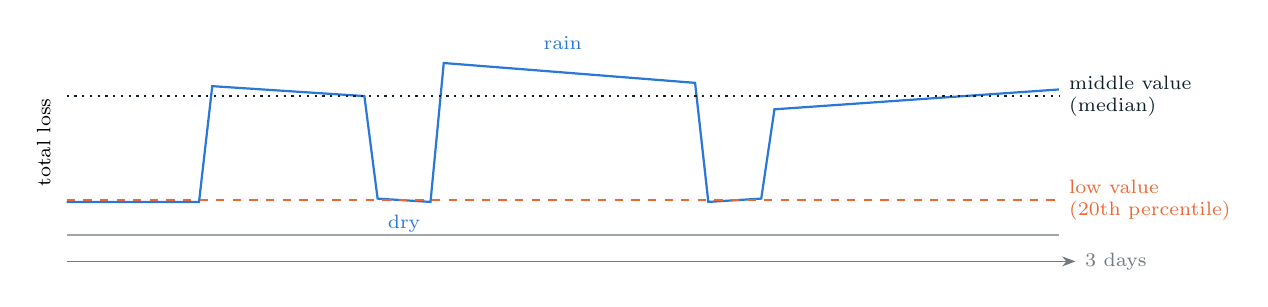
\begin{tikzpicture}[x=0.42cm,y=0.42cm]
  \draw[inkc!40] (0,0) -- (30,0);
  \draw[-{Stealth},inkc!60] (0,-0.8) -- (30.5,-0.8) node[right,font=\scriptsize] {3 days};
  % dry stretches at 1, rainy stretches at 3-6
  \draw[rainc,thick] (0,1) -- (4,1) -- (4.4,4.5) -- (9,4.2) -- (9.4,1.1) -- (11,1) -- (11.4,5.2) -- (19,4.6)
     -- (19.4,1) -- (21,1.1) -- (21.4,3.8) -- (30,4.4);
  \draw[gaugec,thick,dashed] (0,1.05) -- (30,1.05) node[right,font=\scriptsize,align=left] {low value\\(20th percentile)};
  \draw[inkc,thick,dotted] (0,4.2) -- (30,4.2) node[right,font=\scriptsize,align=left] {middle value\\(median)};
  \node[font=\scriptsize,rainc,anchor=south] at (15,5.3) {rain};
  \node[font=\scriptsize,rainc,anchor=north] at (10.2,0.9) {dry};
  \node[font=\scriptsize,rotate=90,anchor=south] at (-0.2,2.8) {total loss};
\end{tikzpicture}
\caption{Illustration (not real data): a link during three mostly rainy days. Because rain filled more than half of the
time, the middle value (dotted) lies on the rainy level. The low value (dashed) still finds the dry level.}
\label{fig:drylevel}
\end{figure}

The old 24-hour median is not thrown away: it becomes the fifth input. When the two disagree, the network can tell that
the recent past was rainy.

\begin{example}[: the extra loss at 08:30 on 25 August]
On sub-link 718 the 3-day low value before 08:30 was 48.70\,dB (the 24-hour median was 48.98). At 08:30 the total
loss was 58.18\,dB, so the extra loss is $58.18-48.70 = 9.48$\,dB. The classical baseline of
Section~\ref{sec:inverse} gave 9.47\,dB: on this ordinary day, the two ways of finding the dry level agree to within
0.01\,dB.
\end{example}

\textbf{Did it work?} Here is how much of the reference rain the AI measured in the hours that followed a mostly
rainy day (more than half of the previous 24 hours rainy). For comparison, the last column shows the same AI at other
times (after a day with less than 10\% rain). The test countries are described in Sections~\ref{sec:italy}
and~\ref{sec:nl}.
\begin{center}\small\setlength{\tabcolsep}{4pt}
\begin{tabular}{lccccc}
\toprule
& share of rainy hours & \multicolumn{3}{c}{AI, after a mostly rainy day} & AI, after a\\
\cmidrule(lr){3-5}
& that follow & & 3-day & + varied & mostly dry\\
Test & a rainy day & 24-h median & low value & training$^{*}$ & day\\
\midrule
Netherlands 2014 & 10\% & 48\% & \textbf{69\%} & -- & 100\%\\
Italy 2022 & 11\% & 64\% & 55\% & \CVfinLongBd & 83\%\\
Italy 2021 & 2\% & 86\% & 77\% & \textbf{\CVfinLongAd} & 77\%\\
\bottomrule
\end{tabular}

\smallskip
{\footnotesize $^{*}$ Section~\ref{sec:varied}: trained on Sweden and on other months of Italy, never on the month judged, with cleaned training answers (Section~\ref{sec:recipe}).}
\end{center}
In the Netherlands the fix works: the shortfall after a rainy day shrank from about half to about a third. In Italy it
did not help: there the AI measures between half and two-thirds of the rain after a rainy day, with either dry level, and the
classical method, which does not use a 24-hour median at all, does no better (62\%). Section~\ref{sec:varied} finds out
why. In short: the dry level is fine; in a long rain the antennas stay wet, the radar we learn from misses the light rain at
its end, and faulty links in the training data had taught the AI that a loss which stays raised for hours is not rain.
Training on more varied weather with cleaned answers (fifth column) fixes this in 2021 and helps clearly in 2022, where these hours come almost
all from one long storm. (An earlier check here said this rain is not lighter than usual. Looked at in 15-minute steps, it is: 1.2
against 2.3\,mm/h on average in 2022, which makes it harder to see under the wet antennas.)

\subsection{How it reads: a magnifying glass sliding along time}
The network's layers are \textbf{convolutions}. A convolution is a small set of weights that slides along the
signal, looking at a few neighbouring minutes at a time, and produces one new number per minute. Picture a magnifying
glass that shows three minutes at once, moved one minute at a time.

Three minutes is short. To see longer patterns without needing a huge number of dials, each layer spaces its three
minutes further apart: the first layer looks at minutes next to each other, the second at minutes 2 apart, then 4, 8,
16, 32, 64 and 128 apart. This trick is called \textbf{dilation}. Stacking eight such layers (each used twice) lets the
final answer depend on the last \textbf{1{,}021 minutes}, about 17 hours. That span is called the
\textbf{receptive field}. Every glass sits at or behind the current minute, never ahead of it; a network built this way
is called a \emph{causal temporal convolutional network} (TCN).

\begin{figure}[h]
\centering
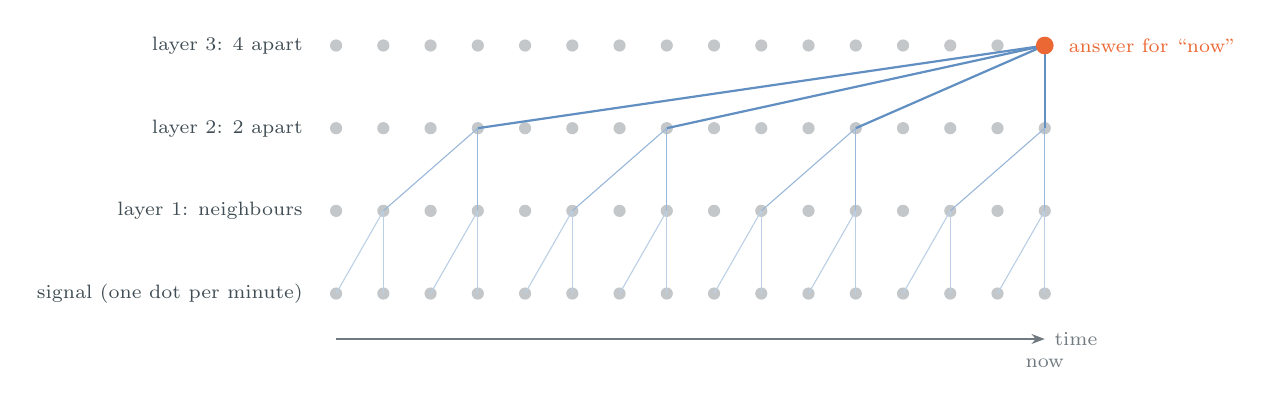
\begin{tikzpicture}[x=0.6cm,y=1.05cm]
  \foreach \row/\lab in {0/{signal (one dot per minute)},1/{layer 1: neighbours},2/{layer 2: 2 apart},3/{layer 3: 4 apart}} {
    \foreach \i in {0,...,15} { \fill[inkc!25] (\i,\row) circle (2.2pt); }
    \node[font=\scriptsize,anchor=east,inkc!80] at (-0.5,\row) {\lab};
  }
  % connections into the last output
  \foreach \s in {15,11,7,3} { \draw[beam!70,thick] (\s,2) -- (15,3); }
  \foreach \t in {15,11,7,3} { \foreach \s in {0,2} { \pgfmathtruncatemacro{\a}{\t-\s} \draw[beam!45] (\a,1) -- (\t,2); } }
  \foreach \t in {15,13,11,9,7,5,3,1} { \foreach \s in {0,1} { \pgfmathtruncatemacro{\a}{\t-\s} \ifnum\a>-1 \draw[beam!30] (\a,0) -- (\t,1); \fi } }
  \fill[gaugec] (15,3) circle (3.2pt);
  \node[font=\scriptsize,anchor=west,gaugec] at (15.3,3) {answer for ``now''};
  \draw[-{Stealth},inkc!60] (0,-0.55) -- (15,-0.55) node[right,font=\scriptsize] {time};
  \node[font=\scriptsize,inkc!60] at (15,-0.85) {now};
\end{tikzpicture}
\caption{How dilation widens the view (simplified: two taps per glass, three layers). Each layer looks further apart, so
the answer for ``now'' (orange) depends on many past minutes but never on future ones. Our real network uses three taps
and eight levels, reaching 1{,}021 minutes into the past.}
\label{fig:tcn}
\end{figure}

\subsection{What it answers: two numbers, then physics}
For each minute the network gives two numbers:
\begin{enumerate}
\item \textbf{The chance it is raining}, $p$, between 0 and 1 (through the sigmoid above). If $p$ is above a
\textbf{threshold} we say ``raining''. We tried thresholds from 0.05 to 0.80 on the validation fortnight and kept the
one with the best MCC: \textbf{0.25}.
\item \textbf{A correction} $c$ in decibels: how much of the extra loss is \emph{not} rain in the air (wet antennas,
the dry level drifting, slow wobbles). It is built to stay between $-1$ and $+4$\,dB, roughly the size wet antennas
really reach.
\end{enumerate}
Then the network steps aside and the physics of Part~1 takes over: the rain-caused loss is $A = \text{extra loss} - c$,
and Equation~\ref{eq:inverse} turns it into mm/h with the ITU coefficients $a$ and $b$ of that link. If $p$ is below the
threshold, the answer is 0.
\[
R = \begin{cases} \left(\dfrac{\text{extra loss} - c}{a\,L}\right)^{1/b} & \text{if } p > 0.25,\\[2ex] 0 & \text{otherwise.}\end{cases}
\]

\begin{oneline}
The AI decides whether it is raining and how much of the loss to blame on things other than rain; the century-old
physics of raindrops still does the conversion into millimetres per hour.
\end{oneline}

\begin{example}[: the AI at 08:30 on 25 August]
The network says $p=0.75$: above 0.25, so ``raining''. Its correction is $c = 4.00$\,dB (at its upper limit; the
classical wet-antenna model said 4.10\,dB). So
\[
A = 9.48 - 4.00 = 5.48\ \text{dB},\qquad
\frac{A}{aL} = \frac{5.48}{0.370\times 1.066} = 13.9,
\]
\[
R = 13.9^{1/0.860} \approx 21.3\ \text{mm/h}.
\]
The classical method gave 20.7\,mm/h for the same minute. Averaged over the 5 minutes around 08:30, the AI says
16.4\,mm/h, the classical method 17.3 and the gauge 14.4.
\end{example}

\begin{figure}[h]
\centering
\begin{tikzpicture}
\begin{groupplot}[group style={group size=1 by 2,vertical sep=0.9cm,xlabels at=edge bottom},
  width=0.92\textwidth,height=4.8cm,xmin=4,xmax=24,xtick={4,6,...,24},grid=major,grid style={inkc!12},
  tick label style={font=\small},label style={font=\small},legend style={font=\scriptsize,draw=none,fill=white,fill opacity=0.85,text opacity=1},legend cell align=left]
\nextgroupplot[ylabel={rain (mm/h)},ymin=0,ymax=24,legend pos=north east]
  \addplot[thick,color=gaugec,forget plot] table[x=hour,y=gauge] {storm.dat};
  \addplot[thick,color=rainc!55,forget plot] table[x=hour,y=R] {storm.dat};
  \addplot[thick,color=inkc,forget plot] table[x=hour,y=ai] {storm_ai.dat};
  \addlegendimage{thick,color=gaugec} \addlegendentry{rain gauge}
  \addlegendimage{thick,color=rainc!55} \addlegendentry{classical method (Part 1)}
  \addlegendimage{thick,color=inkc} \addlegendentry{AI}
\nextgroupplot[ylabel={dB},xlabel={hour of the day (UTC), 25 August 2015},ymin=-1.5,ymax=10,legend pos=north east]
  \addplot[very thin,color=rainc,forget plot] table[x=hour,y=excess] {storm_ai.dat};
  \addplot[thick,color=gaugec,forget plot] table[x=hour,y=corr] {storm_ai.dat};
  \addlegendimage{thick,color=rainc} \addlegendentry{extra loss (over the 3-day dry level)}
  \addlegendimage{thick,color=gaugec} \addlegendentry{AI's correction $c$}
\end{groupplot}
\end{tikzpicture}
\caption{The same storm as Figure~\ref{fig:storm}, now with the AI. Top: rain from the AI (5-minute averages), the
classical method and the gauge 4\,m away. Bottom: what the AI saw (extra loss) and how much of it the AI decided was
not rain in the air. In dry spells the correction stays near 0\,dB; there the rain/no-rain answer keeps the rain at
zero. In the storm the correction climbs to its 4\,dB limit (wet antennas), and only the loss above that is turned into
rain. The AI under-reads the short burst at 17:05 (about 4\,mm/h against the gauge's 12).}
\label{fig:storm_ai}
\end{figure}

\subsection{How it was trained}
\begin{itemize}
\item \textbf{Examples:} the 683 Gothenburg sub-links that passed quality control in Phase~1, over the training
weeks. The ``right answer'' is the weather radar's rain along each link path, available every 5 minutes.
\item \textbf{One round:} 64 pieces of signal, each 2{,}560 minutes long (about 43 hours), picked at random links and
random times. The first 1{,}024 minutes of each piece are only there to fill the network's 17-hour view; they are not
scored.
\item \textbf{Penalties:} the rain/no-rain penalty on every radar minute, and the squared-mistake penalty for the
amount \emph{only on minutes where the radar says it rained}. (Why only those? See ``What went wrong first'' below.)
\item \textbf{Practice with coarse data:} in half the rounds, the signal was first rounded to whole decibels, the way
much operator equipment stores it (Italy's does). This is called \textbf{augmentation}: showing the same examples in
a slightly different form so the network learns not to depend on details that change between networks.
\item \textbf{How long:} 4{,}000 rounds, about one minute on one graphics card (GPU, a chip built for doing many
multiplications at once). Every 250 rounds we checked the validation fortnight and kept the best version.
\item \textbf{Five tries, keep one:} training starts from random dials, and two runs never end up identical (more on this
in Section~\ref{sec:se_results}). So we trained five times and kept the run with the smallest penalty on the validation
fortnight. That choice uses no test data. The kept network has 111{,}890 dials.
\end{itemize}

\subsection{What went wrong first}
Our first designs failed, and how they failed is instructive.
\begin{enumerate}
\item \textbf{Letting the network say the mm/h directly.} It caught rain well, but reported only about half the rain.
The training weeks (June, early July) had light rain; August had heavy storms. When the network meets a signal drop
bigger than anything it practised on, it plays safe and answers something it has seen before. A network that only
learned from examples has no reason to believe the rain can be heavier than in its examples.
\item \textbf{Physics conversion, but an unlimited correction learned on all minutes.} Now it reported a quarter of the
rain. On the many dry minutes it learned that subtracting a lot is always safe, and it carried the habit into storms.
\item \textbf{A dry level that fails after a rainy day.} The 24-hour median of Section~\ref{sec:drylevel}. This did not
show up in Sweden at all; it showed up in Italy and the Netherlands.
\end{enumerate}
The fixes are the design described above: a correction limited to $-1\ldots4$\,dB, the amount learned only when it
rains, and the 3-day low dry level. The physics conversion extrapolates to heavy rain by itself, because the power law
does not care whether the network practised on heavy storms.

\begin{careful}
we made the first two fixes after looking at the Swedish August scores, and the third after looking at the Italian and
Dutch results. So none of the three tests is a perfectly untouched exam any more: in each case we chose part of the
design after seeing how it did there. What we did \emph{not} do is tune numbers on them: the 3-day window and the 20\%
were chosen from reasoning, and nothing was trained on Italian or Dutch data. A truly fresh test needs data we have not
looked at yet, such as another year or another country.
\end{careful}

%==========================================================
\section{Before the results: exactly how we score}
\label{sec:scoring_rules}
%==========================================================

Section~\ref{sec:scores} introduced the scores. Before using them on three countries, here are the exact rules, because
small choices in how scores are counted can make a method look better or worse than it is. Both methods, classical and AI,
are always scored with the same rules, on the same links and the same hours.

\subsection{Two separate exams}
Every test has two parts, and they answer different questions:
\begin{itemize}
\item \textbf{Rain or no rain?} Only the yes/no answer is checked, not the amount. Scores: MCC, share of rain caught,
share of false alarms.
\item \textbf{How much rain?} The method's millimetres per hour are compared with the measured millimetres per hour. Scores:
correlation $r$, typical error (RMSE) and bias.
\end{itemize}
A method can pass one and fail the other. A detector that always says ``raining'' during storms but gets the amount
wrong by half would score well on the first and badly on the second.

\subsection{Rule 1: what counts as ``rain''}
A time step counts as \textbf{rainy} if the reference measured \textbf{at least 0.1\,mm/h} there. Less than that is
too little to matter and is often just noise in the reference itself.

Our methods give an answer every minute, but the references come every 5, 15 or 60 minutes. So for the yes/no exam we
look at the minutes inside each reference period and call the period rainy for the method if \textbf{more than half}
of those minutes were rainy.

\subsection{Rule 2: dry moments are left out of the amount scores}
For the amounts, a time step is only scored if \textbf{the reference or the method} shows at least 0.1\,mm/h. Moments
where both agree it was dry are skipped. Why? Most hours are dry. Every dry hour where both say 0 is a ``perfect''
answer that has nothing to do with measuring rain, and thousands of them would make the typical error look tiny.

\begin{example}[: why dry hours are skipped]
Five hours, reference against method (mm/h):
\begin{center}\small
\begin{tabular}{lccccc}
\toprule
Hour & 1 & 2 & 3 & 4 & 5\\
\midrule
Reference & 0 & 0 & 2.0 & 8.0 & 0.05\\
Method & 0 & 0.3 & 1.5 & 6.0 & 0\\
\midrule
Scored? & no (both dry) & yes (method $\geq$ 0.1) & yes & yes & no (both below 0.1)\\
\bottomrule
\end{tabular}
\end{center}
The three scored mistakes are $+0.3$, $-0.5$ and $-2.0$\,mm/h. Then
\[
\text{RMSE} = \sqrt{\frac{0.3^2 + 0.5^2 + 2.0^2}{3}} = \sqrt{\frac{0.09+0.25+4}{3}} = 1.20\ \text{mm/h},
\]
\[
\text{bias} = \frac{(0.3+1.5+6.0)-(0+2.0+8.0)}{0+2.0+8.0} = -22\%.
\]
Had we scored all five hours, the RMSE would have dropped to 0.93\,mm/h, only because of the two dry hours, though the
method measured the rain no better.
\end{example}

Notice that hour 2 \emph{is} scored: when the method claims rain the reference did not see, that false rain counts as a
mistake. A method cannot hide its false alarms by skipping them.

\subsection{Rule 3: which reference, and how often}
\begin{center}\small
\begin{tabular}{p{2.3cm}p{7.4cm}p{3.9cm}}
\toprule
Where & Reference & Compared every\\
\midrule
Sweden & weather radar, averaged along the link & 5 minutes and 1 hour\\
       & rain gauges within 1\,km of the link & 1 hour\\
Italy & gauge-adjusted radar, averaged along the link & 15 minutes and 1 hour\\
      & rain gauges within 1\,km of the link & 1 hour\\
Netherlands & gauge-adjusted radar, averaged along the link & 1 hour\\
\bottomrule
\end{tabular}
\end{center}
``Averaged along the link'' means: take every radar square the beam crosses and average them, giving more weight to the
squares where the beam travels a longer distance. That is the same thing the link itself measures.

\subsection{No reference is the true rain}
It is tempting to call the gauge ``the truth''. It is not, for this job:
\begin{itemize}
\item \textbf{A gauge measures one spot}, the size of a bucket. The link measures the average along a line that can be
several kilometres long. A storm cell 2\,km wide can soak the gauge and only half the link, or the other way round. So
even a perfect link and a perfect gauge disagree. That is why we only pair a link with gauges within 1\,km of it, and why
we compare hours rather than minutes (over an hour, a passing storm crosses both).
\item \textbf{Radar sees the whole line} but measures echoes high in the air and converts them to rain with a formula of
its own. Plain radar (Sweden) can be off by tens of percent; gauge-adjusted radar (Italy, the Netherlands) has been
corrected with gauges and is better, but still averages over 1\,km squares.
\end{itemize}
So a correlation of 1 is impossible even for a perfect method. As a yardstick: in Sweden, the radar itself agrees with the
gauges at $r = 0.80$ (hourly). A link method scoring around 0.8 against gauges is as close as the radar gets.

\begin{oneline}
We score two things separately (rain or not, and how much), count rain from 0.1\,mm/h, leave out moments where everyone
agrees it was dry, and compare with references that are good but not perfect.
\end{oneline}

%==========================================================
\section{Results in Sweden}
\label{sec:se_results}
%==========================================================

Same links, same month (August 2015), same scores as Section~\ref{sec:scores}.

\begin{center}\small
\begin{tabular}{lcccc}
\toprule
& \multicolumn{2}{c}{\textbf{Rain or no rain}} & \multicolumn{2}{c}{\textbf{How much (hourly, vs gauges)}}\\
\cmidrule(lr){2-3}\cmidrule(lr){4-5}
Method & MCC & caught / false alarms & correlation $r$ & error (RMSE) / bias\\
\midrule
Classical (Part 1) & 0.578 & 71\% / 4.6\% & 0.81 & 1.04\,mm/h / $-6\%$ \\
AI & \textbf{0.615} & 68\% / \textbf{3.2\%} & 0.79 & 1.04\,mm/h / $-20\%$ \\
\midrule
\multicolumn{5}{l}{\emph{Same August data, but rounded to whole decibels first:}}\\
Classical & 0.336 & 82\% / 23\% & 0.85 & 0.82\,mm/h / $+26\%$ \\
AI & \textbf{0.568} & 65\% / \textbf{3.9\%} & 0.80 & 0.96\,mm/h / \textbf{$-15\%$} \\
\bottomrule
\end{tabular}
\end{center}

Reading the table:
\begin{itemize}
\item \textbf{Rain or no rain:} the AI is better. It raises fewer false alarms (3.2\% of dry periods instead of
4.6\%) at the cost of missing slightly more light rain. And it does this without looking into the future.
\item \textbf{Amounts:} the classical method is better. The AI follows the ups and downs about as well (correlation 0.79
against 0.81, same typical error), but it measures a fifth too little rain, against 6\% too little for the classical
method. Against the radar (not in the table) it is also slightly behind: hourly $r$ 0.71 against 0.76.
\item \textbf{Coarse data:} this is the clearest win. Rounded to whole decibels, the classical detector panics (23\%
false alarms, because 1-dB steps look like jumpiness), while the AI barely changes.
\end{itemize}

\subsection{Is the AI just lucky?}
Training starts from random dials, so two training runs never give exactly the same network. Here are all five training
runs of the same design, with different random starts (``seeds''):
\begin{center}\small
\begin{tabular}{lcc}
\toprule
& average of 5 runs & worst -- best \\
\midrule
MCC & 0.619 & 0.612 -- 0.637 \\
hourly correlation with gauges & 0.79 & 0.77 -- 0.84 \\
hourly error vs gauges (RMSE) & 1.05\,mm/h & 0.90 -- 1.15 \\
bias vs gauges & $-22\%$ & $-32\%$ -- $-6\%$ \\
\bottomrule
\end{tabular}
\end{center}
So: the better rain detection is solid (every run beats 0.578). The amounts are not: one run under-measures by only
6\%, another by 32\%, with nothing but the random start to tell them apart. The run we kept (chosen on validation, not on
these numbers) sits in the middle, at $-20\%$. Picking the run that happens to score best in August would have made the
AI look much better than it is. Section~\ref{sec:why_runs} finds why the runs differ: not in \emph{when} they say it rains,
but in how strongly they turn a decibel into millimetres, which each run learns from a handful of heavy Swedish minutes.
Training on more varied rain brings them together (Section~\ref{sec:cv}).

\subsection{Which design choices mattered?}
Removing one ingredient at a time (an \textbf{ablation}) shows what each does:
\begin{center}\footnotesize
\begin{tabular}{p{6.3cm}cccc}
\toprule
Version (one training run each) & MCC & $r$ vs gauges & bias vs gauges & MCC, 1-dB data\\
\midrule
Full design & 0.615 & 0.79 & $-20\%$ & 0.568\\
Network says mm/h directly (no physics conversion) & 0.618 & 0.75 & $-19\%$ & 0.550\\
No practice on 1-dB rounded data & 0.634 & 0.79 & $-27\%$ & 0.481\\
\bottomrule
\end{tabular}
\end{center}
The practice on rounded data clearly matters for coarse data (0.481 without it, against 0.568). For the physics
conversion the picture is less clear than we first thought: with the final design, a network that outputs mm/h
directly does about as well \emph{in Sweden}. Differences this small are within the spread between training runs shown
above. The physics conversion was what rescued our first designs from heavy under-measurement; whether it still helps
abroad, we have not tested.

\begin{oneline}
In Sweden the AI detects rain better than the classical method, works live, and copes far better with coarse data, but
it measures about a fifth too little rain, and how much too little changes from one training run to the next.
\end{oneline}

%==========================================================
\section{A harder exam: Italy}
\label{sec:italy}
%==========================================================

A method that only works in the city where it was trained is of little use for Algeria. So we took the network trained
in Gothenburg and, \textbf{without any change}, ran it on a completely different network: the Lepida network in
Emilia-Romagna, northern Italy (the OpenRainER dataset). Using a model on a place it never learned from is called a
\textbf{zero-shot} test. The classical method was also used with its Swedish settings.

Almost everything is different there:
\begin{center}\small
\begin{tabular}{p{3.4cm}p{4.6cm}p{5.6cm}}
\toprule
& Sweden (training) & Italy (test)\\
\midrule
Frequencies & 7.5 -- 39\,GHz & only 24.5 -- 25.6\,GHz\\
Link lengths & half under 2.3\,km, up to 15\,km & up to 25\,km (after quality control: up to 9\,km)\\
Landscape & flat coastal city & plains, hills and Apennine mountains\\
Rounding of readings & 0.1\,dB & 1\,dB\\
Period & summer 2015 & May -- September 2021 and 2022\\
\bottomrule
\end{tabular}
\end{center}

The references in Italy are good: a \textbf{gauge-adjusted radar} (radar maps corrected with hundreds of rain gauges,
every 15 minutes, 1\,km squares) and 22--23 gauges standing within 1\,km of a link. One detail had to be checked: the files
do not say whether a 15-minute value is labelled at the start or the end of its 15 minutes. We tried both on the classical
estimates; ``end'' fits clearly better (correlation 0.25 against 0.18), and we used it for both methods.

\begin{careful}
we applied the same quality-control rule as in Sweden (drop a sub-link if it has less than half its data or is flagged
``wet'' more than 30\% of the time by the classical detector). With 1-dB readings the classical detector flags many
links as almost always wet, so only 81 of 302 sub-links (2021) and 72 of 302 (2022) survived. Both methods are scored
on exactly the same surviving links, but the rule judges links with one of the two methods being compared.
Section~\ref{sec:neighbours} tries the fairer alternative: keep every link that has data, and let a neighbour check
catch the bad ones.
\end{careful}

\begin{center}\footnotesize
\begin{tabular}{llcccc}
\toprule
Season & Method & MCC & caught / false alarms & vs radar (hourly): $r$ / bias & vs gauges (hourly): $r$ / bias\\
\midrule
2021 & classical & 0.25 & 75\% / 16.7\% & 0.22 / $+64\%$ & 0.45 / $+39\%$\\
     & AI        & \textbf{0.51} & 57\% / \textbf{1.8\%} & \textbf{0.70} / $\mathbf{-5\%}$ & \textbf{0.74} / $\mathbf{-3\%}$\\
2022 & classical & 0.27 & 70\% / 16.3\% & 0.12 / $+132\%$ & 0.31 / $+64\%$\\
     & AI        & \textbf{0.50} & 51\% / \textbf{1.9\%} & \textbf{0.68} / $\mathbf{-7\%}$ & \textbf{0.81} / $\mathbf{-10\%}$\\
\bottomrule
\end{tabular}
\end{center}

The AI wins clearly on both exams. The classical detector raises false alarms on one dry period in six, the AI on one in
fifty. For amounts, the AI's hourly correlation with the gauges (0.74 and 0.81) is as good as in Sweden, and its total is
within 10\% of the truth, while the classical method's correlations fall to 0.12--0.45 and it measures far too much.
Why does the classical method collapse?

\subsection{A few broken hours spoil the average}
The correlation in the table is computed over all links and hours together (``pooled''). Correlation is very sensitive to
a few wild values: one hour where a link claims 400\,mm/h while the radar says 2 can drag it down more than a thousand good
hours lift it up. So we also computed it the other way: for \emph{each link on its own}, how well do its hours follow the
radar? And we counted the impossible hours (more than 100\,mm/h for a whole hour, which essentially never happens there).

\begin{center}\small
\begin{tabular}{llcc}
\toprule
Season & Method & typical link's $r$ (median) & impossible hours ($>$100\,mm/h)\\
\midrule
2021 & classical & 0.84 & 35\\
     & AI        & 0.82 & 0\\
2022 & classical & 0.79 & 124\\
     & AI        & 0.79 & 0\\
\midrule
\multicolumn{2}{l}{Sweden, for comparison (classical / AI)} & 0.88 / 0.87 & \\
\bottomrule
\end{tabular}
\end{center}

This explains it. \textbf{The typical Italian link follows the radar almost as well as a Swedish one} (about 0.8
against 0.88), with both methods. What ruins the classical pooled numbers is a small number of hours where a link
misbehaves, for example a sudden drop of the signal caused by equipment rather than rain, read as a cloudburst. The
AI produced none at all.

An earlier version of our network, which had only the 24-hour median as its dry level, still produced 8 and 19 such
hours, and its pooled correlation was only 0.33. Adding the second dry level removed them. We think we know why, but
have not proven it: a signal that jumps to a new level and stays there (equipment) moves the 24-hour median and the
3-day low value very differently from rain, which comes and goes. With both in front of it, the network can tell the
two apart.

\begin{figure}[h]
\centering
\begin{tikzpicture}
\begin{axis}[width=0.95\textwidth,height=5.2cm,xmin=11,xmax=14.5,ymin=0,ymax=36,grid=major,grid style={inkc!12},
  xtick={11,11.5,...,14.5},xticklabels={11:00,11:30,12:00,12:30,13:00,13:30,14:00,14:30},
  xlabel={time of day (UTC), 8 June 2021},ylabel={rain (mm/h, 15-min average)},
  tick label style={font=\small},label style={font=\small},
  legend style={font=\scriptsize,draw=none,fill=white,fill opacity=0.85,text opacity=1},legend cell align=left,legend pos=north east]
  \addplot[thick,color=gaugec,mark=*,mark size=1.3pt] table[x=hour,y=gauge] {italy_storm.dat};
  \addlegendentry{rain gauge, 84\,m from the link}
  \addplot[thick,color=radarc,mark=square*,mark size=1.3pt] table[x=hour,y=radar] {italy_storm.dat};
  \addlegendentry{gauge-adjusted radar along the link}
  \addplot[thick,color=rainc!55,mark=triangle*,mark size=1.6pt] table[x=hour,y=classical] {italy_storm.dat};
  \addlegendentry{classical method}
  \addplot[thick,color=inkc,mark=diamond*,mark size=1.6pt] table[x=hour,y=ai] {italy_storm.dat};
  \addlegendentry{AI (trained in Sweden only)}
\end{axis}
\end{tikzpicture}
\caption{A short cloudburst in Italy (sub-link 154, 2.1\,km, 24.6\,GHz). This storm was picked by a fixed rule (the
closest link--gauge pair that saw more than 20\,mm/h), not because it looks good. Both link methods are shown after the
neighbour check of Section~\ref{sec:neighbours}. Storm totals: gauge 11.0\,mm, AI 6.8\,mm, classical 6.2\,mm, radar
4.4\,mm. A storm lasting half an hour over a few square kilometres is exactly the kind
radar smooths away and flash floods come from.}
\label{fig:italy}
\end{figure}

%==========================================================
\section{A different kind of data: the Netherlands}
\label{sec:nl}
%==========================================================

\subsection{Minimum and maximum instead of averages}
Gothenburg's links report the signal every 10 seconds, and Italy's every minute. Many operators keep far less. The Dutch
operator, like many, stored only \textbf{two numbers per 15 minutes}: the weakest and the strongest received level in
that quarter of an hour. This is called \textbf{min/max data}.

\begin{figure}[h]
\centering
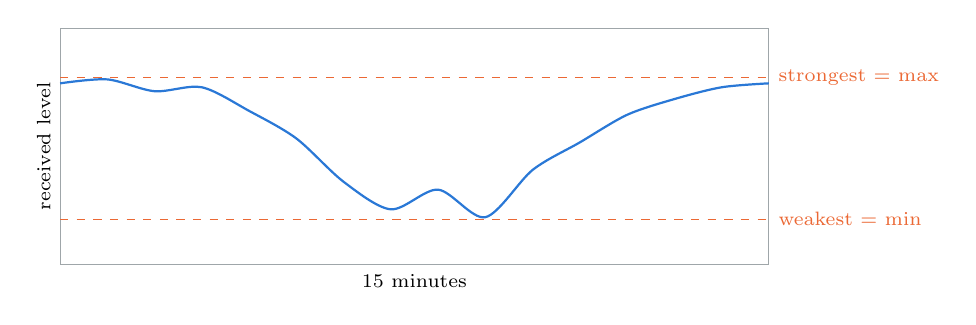
\begin{tikzpicture}[x=0.6cm,y=0.5cm]
  \draw[inkc!40] (0,0) rectangle (15,6);
  \draw[rainc,thick] plot[smooth,tension=0.5] coordinates {(0,4.6) (1,4.7) (2,4.4) (3,4.5) (4,3.9) (5,3.2) (6,2.1) (7,1.4) (8,1.9) (9,1.2) (10,2.4) (11,3.1) (12,3.8) (13,4.2) (14,4.5) (15,4.6)};
  \draw[gaugec,dashed] (0,4.75) -- (15,4.75) node[right,font=\scriptsize] {strongest = max};
  \draw[gaugec,dashed] (0,1.15) -- (15,1.15) node[right,font=\scriptsize] {weakest = min};
  \node[font=\scriptsize,anchor=north] at (7.5,0) {15 minutes};
  \node[font=\scriptsize,rotate=90,anchor=south] at (0,3) {received level};
\end{tikzpicture}
\caption{What min/max data keeps. The real signal (blue) wanders during 15 minutes; only its weakest and strongest
values are stored. Everything in between is thrown away.}
\label{fig:minmax}
\end{figure}

Our network was built for minute-by-minute data, so it cannot read this directly. But we can turn the Swedish data into
the Dutch format: for every 15 minutes, take the weakest and strongest of the ninety 10-second readings (and, in half of
the practice rounds, round them to whole decibels first, like the Dutch Nokia equipment). We trained a min/max version of
the same network on that, with the same weeks and the same rules as before. Its view reaches back 63 hours.

For comparison we built a classical min/max method in the style of \textbf{RAINLINK}, the algorithm developed at the Dutch
meteorological institute (KNMI) and Wageningen University for this kind of data: call it rain if the weakest level falls more than 1.75\,dB below the
24-hour reference, subtract a fixed 2.3\,dB for wet antennas, and mix the rain from the weakest and strongest readings
as $0.33\times$ (from weakest) $+ 0.67\times$ (from strongest). The 1.75\,dB and the 2.3\,dB were chosen on Swedish June--July
data. (Real RAINLINK also compares each link with its neighbours to throw out links that drop alone; we test our own
version of that, for both methods, in Section~\ref{sec:neighbours}.)

\subsection{The test}
We then ran both, unchanged, on the Netherlands from 1 June to 22 August 2014: 1{,}081 sub-links (after the same quality
rule, plus dropping links below 10\,GHz, which rain barely affects), 15--58\,GHz, 0.1 to 16\,km long. The reference is
KNMI's gauge-adjusted radar, one value per hour per 1\,km square, averaged along each link. Polarisation is not in the
Dutch files, so we assumed vertical.

\begin{center}\footnotesize
\begin{tabular}{lccccc}
\toprule
Method & MCC (hourly) & $r$ (pooled) & RMSE & bias & typical link's $r$ / impossible hours\\
\midrule
Classical min/max & \textbf{0.63} & 0.16 & 8.7\,mm/h & $+54\%$ & 0.79 / 219\\
AI min/max        & 0.55 & \textbf{0.50} & \textbf{2.5\,mm/h} & \textbf{$+16\%$} & 0.77 / \textbf{26}\\
\bottomrule
\end{tabular}
\end{center}

Here the classical method detects rain better (hourly MCC 0.63 against 0.55). For amounts, the same story as Italy: the
typical link works with both methods (0.77--0.79), the classical method produces many impossible hours that destroy its
pooled score, and the AI produces eight times fewer, though not none. Split by equipment maker, the AI does better on
Nokia links (1-dB readings, bias $+10\%$) than on NEC links (0.1-dB readings, $+41\%$).

\begin{figure}[h]
\centering
\begin{tikzpicture}
\begin{axis}[width=0.98\textwidth,height=5.4cm,xmin=-1,xmax=83,ymin=0,ymax=26,
  xlabel={day (1 June -- 22 August 2014)},ylabel={rain (mm/day)},
  xtick={0,30,61},xticklabels={1 June,1 July,1 August},grid=major,grid style={inkc!12},
  tick label style={font=\small},label style={font=\small},
  legend style={font=\scriptsize,draw=none,fill=white,fill opacity=0.85,text opacity=1},legend cell align=left,legend pos=north west]
  \addplot[ycomb,line width=2.2pt,color=radarc!55,forget plot] table[x=day,y=radar] {nl_daily.dat};
  \addlegendimage{line width=2.2pt,color=radarc!55}
  \addlegendentry{KNMI radar}
  \addplot[only marks,mark=triangle*,mark size=1.8pt,color=rainc!70] table[x=day,y=classical] {nl_daily.dat};
  \addlegendentry{classical min/max}
  \addplot[only marks,mark=*,mark size=1.4pt,color=inkc] table[x=day,y=ai] {nl_daily.dat};
  \addlegendentry{AI min/max}
\end{axis}
\end{tikzpicture}
\caption{Daily rain averaged over every Dutch link with enough data (1{,}908 sub-links), after the neighbour check of
Section~\ref{sec:neighbours}. Day to day both methods follow the radar well (correlation 0.90 classical, 0.94 AI). Over the
whole summer the classical method adds up to 223\% of the radar's rain and the AI to 132\%: with every link included,
both measure too much, the classical method far more.}
\label{fig:nl}
\end{figure}

\begin{oneline}
Trained only in Sweden, the AI ran in Italy and the Netherlands with no retraining; the typical link worked in both
countries, the AI made no absurd readings in Italy and far fewer than the classical method in the Netherlands, where a guard
against misbehaving links is still needed.
\end{oneline}

%==========================================================
\section{Catching misbehaving links: the neighbour check}
\label{sec:neighbours}
%==========================================================

So far, a small number of links that misbehave, for example a signal that suddenly drops because of the equipment, have
spoiled the averages in Italy and the Netherlands. And in Italy we kept only the links the classical detector liked. Both
problems have the same natural fix, used by the Dutch RAINLINK method: \textbf{ask the neighbours}.

\subsection{The idea}
Rain falls from clouds that are kilometres wide. If it really rains on one link, other links close by almost always feel it
too, within minutes. A link that claims a storm while every link around it stays dry is far more likely broken than wet.

Our rule, applied in exactly the same way to the classical method and to the AI:
\begin{enumerate}
\item \textbf{Neighbours} of a link are the other links whose middle point is within \textbf{10\,km} of its own. (The two
directions of one physical link do not count as each other's neighbours: they share the same equipment and the same air,
so they would fail together.)
\item A link's rain counts only if at least \textbf{one neighbour also reports rain} (0.1\,mm/h or more) within
\textbf{15 minutes before or after}. Otherwise it is set to zero.
\item If \emph{no} neighbour has any data at that moment, the link cannot be checked and is left alone.
\end{enumerate}
We fixed 10\,km and 15 minutes from the size and speed of storms (a storm moving at 40\,km/h crosses 10\,km in 15 minutes),
before looking at any results. The price is a delay: a warning may need up to 15 minutes to be confirmed by a neighbour.

\begin{example}[: three links, one storm, one fault]
Links A and B are 4\,km apart; link C is 6\,km from both. At 14:00 link A reports 12\,mm/h. Link B reports rain from 14:10.
Link A's rain counts: B confirms it within 15 minutes. At 20:00 link C reports 40\,mm/h for an hour while A and B, both
working, report nothing from 19:45 to 21:15. C's rain is set to zero: no neighbour confirms it.
\end{example}

\subsection{Results on the same links as before}
First on exactly the links of the previous sections, to see what the check alone does. ``Impossible hours'' are hours with
more than 100\,mm/h, as in Section~\ref{sec:italy}.
\begin{center}\footnotesize
\begin{tabular}{llccc}
\toprule
Test (links) & Method & MCC & impossible hours & bias vs gauges / radar\\
\midrule
Sweden (683) & classical & 0.578 $\to$ 0.581 & 0 $\to$ 0 & $-6\%$ $\to$ $-6\%$\\
             & AI        & 0.617 $\to$ 0.622 & 0 $\to$ 0 & $-19\%$ $\to$ $-19\%$\\
Italy 2021 (81) & classical & 0.251 $\to$ 0.254 & 35 $\to$ 26 & $+39\%$ $\to$ $+28\%$\\
                & AI        & 0.509 $\to$ 0.518 & 0 $\to$ 0 & $-3\%$ $\to$ $-7\%$\\
Italy 2022 (72) & classical & 0.269 $\to$ 0.271 & 124 $\to$ 77 & $+64\%$ $\to$ $+36\%$\\
                & AI        & 0.502 $\to$ 0.506 & 0 $\to$ 0 & $-10\%$ $\to$ $-14\%$\\
Netherlands (1{,}081) & classical & 0.626 $\to$ 0.632 & 219 $\to$ 163 & $+54\%$ $\to$ $+43\%$\\
                      & AI        & 0.547 $\to$ 0.562 & 26 $\to$ 16 & $+16\%$ $\to$ $+12\%$\\
\bottomrule
\end{tabular}
\end{center}
(Bias is against gauges for Sweden and Italy, against radar for the Netherlands. The AI's Swedish MCC is 0.617 here rather
than 0.615 because it is scored only where the link has data, like the classical method.)

The check helps both methods everywhere, a little: rain detection never gets worse, and impossible hours drop by a quarter
to a half. It does not remove them all. A broken classical link is often ``confirmed'' by a neighbour that is itself
raising a false alarm, which happens easily when the classical detector raises false alarms on one dry period in six. In
Sweden, where links are dense (a typical link has 192 neighbours) and well behaved, the check removes under 2\% of rainy
minutes and changes almost nothing. In Italy, where a typical link has only 6--7 neighbours, it removes about a fifth of the
rainy minutes; the AI's amounts drop by only about 5\%, so most of what it removed was little or no rain, but some real rain
went too.

\subsection{Keeping every link}
Now the fairer filter: keep \textbf{every link that has data at least half of the time}, and let the neighbour check do the
cleaning. In Italy that means 281 and 267 sub-links instead of 81 and 72; in the Netherlands 1{,}908 instead of 1{,}081
(still dropping links below 10\,GHz).
\begin{center}\footnotesize\setlength{\tabcolsep}{4pt}
\begin{tabular}{llcccc}
\toprule
Test (links) & Method, with neighbour check & MCC & impossible hours & $r$ vs gauges & bias vs gauges\\
\midrule
Italy 2021 (281) & classical & 0.158 & 43 & 0.45 & $+76\%$\\
                 & AI        & \textbf{0.449} & \textbf{0} & \textbf{0.72} & $\mathbf{+3\%}$\\
Italy 2022 (267) & classical & 0.168 & 106 & 0.38 & $+49\%$\\
                 & AI        & \textbf{0.443} & \textbf{5} & \textbf{0.69} & $-16\%$\\
\midrule
& & & & $r$ vs radar & bias vs radar\\
\midrule
Netherlands (1{,}908) & classical & 0.463 & 199 & 0.19 & $+128\%$\\
                      & AI        & \textbf{0.484} & \textbf{19} & \textbf{0.52} & $\mathbf{+34\%}$\\
\bottomrule
\end{tabular}
\end{center}

Two things stand out:
\begin{itemize}
\item \textbf{The extra links are worse links.} With every link included, both methods score lower than on the hand-picked
set (Italian rain detection 0.45 instead of 0.52 for the AI; Dutch 0.48 instead of 0.56). The old filter was unfair, but it
was throwing out links that deserved it. The neighbour check alone does not replace it.
\item \textbf{The AI copes much better with bad links.} On every link, it still detects rain about three times better than
the classical method in Italy, has almost no impossible hours, and stays within 3--16\% of the Italian gauges, while the
classical method measures half to three-quarters too much. In the Netherlands the AI now also beats the classical method at
detecting rain (0.48 against 0.46).
\end{itemize}
For a real operator network, where nobody hand-picks the links, this second table is the honest picture. What it calls for
is a fair way to judge each link from its own behaviour, instead of throwing out links with the classical detector.

\subsection{A reliability score for each link}
\label{sec:reliability}
The score looks only at the raw signal, never at the rain worked out by either method, so it cannot favour one of them.
Every 15 minutes we compare the link's total loss with its own dry level (the 3-day low value of
Section~\ref{sec:drylevel}). If it is at least \textbf{1.5\,dB} above, we call that 15 minutes a \textbf{signal event}:
something is weakening the beam. Then two questions about each link:
\begin{enumerate}
\item \textbf{Does it rain alone?} For each of its events, did at least one of its \textbf{5 nearest neighbours} (within
10\,km) also have an event within 15 minutes? If more than half of its events had no such company (and it had at least 8
events, enough to judge), the link is dropped.
\item \textbf{Is it always ``raining''?} If the link is in an event more than \textbf{20\%} of the time, it is dropped. In
these climates it rains far less than a fifth of the time; a beam that is weakened that often is drifting or faulty.
\end{enumerate}
Links with at least half their data that pass both questions are kept.

\begin{example}[: one link judged]
Over a summer, a link has 40 signal events. For 30 of them at least one of its five nearest neighbours also had an event
within 15 minutes; 10 had no company. Unconfirmed share: $10/40 = 25\%$, below one half, so the first question passes. Its
40 events are 40 of its roughly 14{,}000 quarter-hours of data, 0.3\% of the time, far below 20\%. The link is kept. A link
whose signal drops every other evening while its neighbours stay calm would have most of its events unconfirmed and be
dropped.
\end{example}

\textbf{How we chose the numbers.} We set them on Swedish June--July data only, where we could check them against the radar
without touching any test month. Our first version asked ``any neighbour within 10\,km''. In Gothenburg a typical link has
192 neighbours that close, and by pure chance one of them is almost always having an event, so almost nothing was ever
judged lonely. Asking only the 5 nearest, and adding the 20\% question, fixed that. On the Swedish June--July data, the
final score drops 69 of 728 sub-links. It agrees with the old rule on 40 of the 45 that rule dropped, and drops 29 more.
Are those 29 really bad? Their raw signal follows the radar with a typical correlation of 0.33, as poorly as the links
both rules drop (0.32), against 0.58 for the links kept. So yes.

\textbf{Results.} The same three link sets, both methods with the neighbour check:
\begin{center}\footnotesize\setlength{\tabcolsep}{4pt}
\begin{tabular}{lllccc}
\toprule
Test & Links & Method & MCC & $r$ / bias$^{*}$ & impossible hours\\
\midrule
Italy 2021 & old rule (81) & AI & 0.518 & 0.75 / $-7\%$ & 0\\
           & all with data (281) & AI & 0.449 & 0.72 / $+3\%$ & 0\\
           & \textbf{reliability score (196)} & AI & \textbf{0.521} & \textbf{0.78} / $-6\%$ & 0\\
           & reliability score (196) & classical & 0.186 & 0.47 / $+47\%$ & 37\\
\midrule
Italy 2022 & old rule (72) & AI & 0.506 & 0.84 / $-14\%$ & 0\\
           & all with data (267) & AI & 0.443 & 0.69 / $-16\%$ & 5\\
           & \textbf{reliability score (194)} & AI & \textbf{0.508} & 0.72 / $-20\%$ & 2\\
           & reliability score (194) & classical & 0.193 & 0.44 / $+23\%$ & 98\\
\midrule
Netherlands & old rule (1{,}081) & AI & 0.562 & 0.53 / $+12\%$ & 16\\
            & all with data (1{,}908) & AI & 0.484 & 0.52 / $+34\%$ & 19\\
            & \textbf{reliability score (1{,}653)} & AI & 0.508 & \textbf{0.55} / $+20\%$ & 18\\
            & reliability score (1{,}653) & classical & 0.517 & 0.22 / $+52\%$ & 180\\
\bottomrule
\end{tabular}

\smallskip
$^{*}$ against gauges in Italy, against the radar in the Netherlands.
\end{center}

\begin{itemize}
\item \textbf{Many more links, same quality, in Italy.} The score keeps 196 and 194 Italian sub-links, more than twice as
many as the old rule, and the AI detects rain as well as on the hand-picked set (0.52 and 0.51). In 2021 it even agrees
better with the gauges (0.78). In 2022 the gauge agreement stays below the old set's (0.72 against 0.84): some of the
extra links are still weaker.
\item \textbf{A middle way in the Netherlands.} 1{,}653 sub-links, in between ``everything'' and the old set, and in between
on rain detection too; the hourly correlation with the radar is the best of the three.
\item \textbf{It does not rescue the classical method.} On the reliable links the classical method still raises too many
false alarms in Italy (MCC 0.19) and keeps many impossible hours. Its problem there is its detector on 1-dB data, not
bad links.
\end{itemize}

\begin{oneline}
Checking each link's rain against its neighbours helps both methods; judging each link by whether its signal drops alone or
all the time lets us keep two to three times more Italian links than hand-picking, with the AI scoring as well as before.
\end{oneline}

%==========================================================
\section{Teaching the AI with more varied weather}
\label{sec:varied}
%==========================================================

Two questions were left open above. Why does the AI still measure too little rain after a rainy day in Italy
(Section~\ref{sec:drylevel})? And why do training runs that agree on \emph{whether} it rains disagree so much on
\emph{how much} (Section~\ref{sec:se_results})? We first looked for the causes, then tried fixes, and kept the test months
untouched throughout.

\subsection{Why the training runs disagree on amounts}
\label{sec:why_runs}
A run's rain total can be wrong in three ways: it calls rain ``dry'' (missed rain), it calls a dry moment ``rain'' (false
rain), or it says ``rain'' at the right moments but with the wrong strength. We split the total of each of the five runs
of Section~\ref{sec:se_results} into these three parts, against the radar, on the July validation weeks and on the
August test month:
\begin{center}\footnotesize\setlength{\tabcolsep}{5pt}
\begin{tabular}{cccccc}
\toprule
& \multicolumn{2}{c}{\textbf{July (validation)}} & \multicolumn{3}{c}{\textbf{August (test)}}\\
\cmidrule(lr){2-3}\cmidrule(lr){4-6}
Run & bias & strength when it says rain & bias & strength & missed / false rain\\
\midrule
\SeedRows
\bottomrule
\end{tabular}
\end{center}
(``Strength'' is the run's rain divided by the radar's, at the moments when both say it rains; 1.00 is perfect. The
missed and false columns are shares of the radar's total.)

Three things stand out:
\begin{itemize}
\item \textbf{It is the strength, not the switch.} All runs miss about the same rain (10--12\%) and add about the same
false rain. What differs is how strongly they convert a decibel into millimetres: from 0.69 to 0.89 of the radar in August.
Fixing the rain/no-rain threshold at the same value for every run does not change this.
\item \textbf{July tells us about August.} A run that reads high in July also reads high in August: the correlation between
the two columns of bias is \SeedValTestR. So the spread is a property of each trained network, not bad luck in August.
\item \textbf{All runs read lower in August than in July}, by 15 to 20 points. August 2015 had more heavy downpours, and the
strength is learned mostly from the few heavy minutes of six weeks in one city. Each run fits those few minutes a little
differently.
\end{itemize}
That last point is the cause: too little and too uniform training rain. The cure we expected was more varied rain.

\subsection{What a long rain looks like to a link}
\label{sec:may6}
The Italian ``after a mostly rainy day'' hours are not spread over the summer. In 2022, 85\% of them come from a single
storm: a day and a half of steady rain on 5--7 May over the Apennine hills. Figure~\ref{fig:may6} shows one link through it,
next to a rain gauge 508\,m away.

\begin{figure}[h]
\centering
\begin{tikzpicture}
\begin{groupplot}[group style={group size=1 by 2,vertical sep=1.5cm,xlabels at=edge bottom},
  width=0.95\textwidth,height=4.6cm,xmin=0,xmax=60,grid=major,grid style={inkc!12},
  xtick={0,12,24,36,48,60},xticklabels={{5 May\\12:00},{6 May\\00:00},{6 May\\12:00},{7 May\\00:00},{7 May\\12:00},{8 May\\00:00}},
  xticklabel style={align=center,font=\scriptsize},
  tick label style={font=\small},label style={font=\small},
  legend style={font=\scriptsize,draw=none,fill=white,fill opacity=0.85,text opacity=1},legend cell align=left]
\nextgroupplot[ylabel={rain (mm/h)},ymin=0,ymax=4.5,legend pos=north east]
  \addplot[thick,color=gaugec,mark=*,mark size=1pt] table[x=hour,y=gauge] {may6.dat};
  \addlegendentry{rain gauge}
  \addplot[thick,color=radarc] table[x=hour,y=radar] {may6.dat};
  \addlegendentry{radar along the link}
  \addplot[thick,color=inkc,dashed] table[x=hour,y=ai_se] {may6.dat};
  \addlegendentry{AI, Sweden only}
  \addplot[thick,color=rainc] table[x=hour,y=ai_cv] {may6.dat};
  \addlegendentry{AI, varied training (never saw May)}
\nextgroupplot[ylabel={dB},xlabel={hourly averages (UTC)},ymin=0,ymax=6,legend pos=north east]
  \addplot[thick,color=inkc] table[x=hour,y=excess] {may6.dat};
  \addlegendentry{extra loss above the dry level}
  \addplot[thick,color=radarc,dashed] table[x=hour,y=expected] {may6.dat};
  \addlegendentry{loss the radar's rain should cause}
\end{groupplot}
\end{tikzpicture}
\caption{The long storm of 5--7 May 2022 on sub-link 182\_1 (5.3\,km, 24.6\,GHz). Top: rain. Bottom: what the link
measured. Storm totals: gauge \Maygauge\,mm, radar \Mayradar\,mm, AI trained on Sweden only \Mayaise\,mm, AI with varied
training \Mayaicv\,mm.}
\label{fig:may6}
\end{figure}

What the figure, and the same numbers for every link, show:
\begin{enumerate}
\item \textbf{The dry level is not the problem.} In every group of Italian rainy hours, the 3-day low value is at or a little below (by
0.1--0.2\,dB, and up to 0.9\,dB in the long storm) the level the link has when the radar says it is dry. It is never too
high, so it cannot be what makes the AI read too little.
\item \textbf{The link sees more than the rain.} While it rains, the extra loss is the rain's share plus a steady 1.5--2\,dB
more: water on the antenna covers, which stay wet in a long rain (the wet antenna of Section~\ref{sec:fakes}).
\item \textbf{The extra loss lasts a whole day after the radar stops} (6 May evening to 7 May noon). The gauge shows why:
light rain, 0.2--1.2\,mm/h, kept falling. The radar, looking from far above, saw almost none of it.
\item \textbf{The AI gives up.} After about twelve hours of raised loss, the AI reports almost nothing, even at hours when
the radar shows 2--4\,mm/h. To a single link, ``my loss has been raised for half a day'' looks like a faulty or drifting link, and
our training data are full of those. That is what the AI learned.
\end{enumerate}
So the cause is not one bug. Three things push the same way: a long rain wets the antennas, the radar we train on misses the
light rain at its end (so the training answer says ``dry'' while the link is still wet), and faulty links teach that a
loss which stays raised for hours is not rain.

\subsection{Trying fixes, one Italian summer at a time}
Each fix was trained five times (seeds 0--4) on Sweden June--July, plus Italy 2021 where stated, and tested on what it never
saw: Sweden in August and Italy in 2022. ``Rain after a mostly rainy day'' is measured here in 15-minute steps, which is
stricter than the hourly table of Section~\ref{sec:drylevel}.
\begin{center}\footnotesize\setlength{\tabcolsep}{3.5pt}
\begin{tabular}{p{5.1cm}ccccc}
\toprule
& \multicolumn{2}{c}{\textbf{Sweden, August}} & \multicolumn{3}{c}{\textbf{Italy 2022}}\\
\cmidrule(lr){2-3}\cmidrule(lr){4-6}
& & bias vs gauges, & total bias, & rain after a & rain after a\\
Training & MCC & 5 runs & 5 runs & dry day & mostly rainy day\\
\midrule
\ExpRows
\bottomrule
\end{tabular}
\end{center}
\begin{itemize}
\item \textbf{One Italian summer fixes most of the spread.} Five runs that disagreed by 47 points on Italy's 2022 total
now agree within 7 to 12 points, and in Sweden within 5 to 17 points instead of 26. Rain detection in Sweden improves too
(MCC 0.65 against 0.62), even though no Swedish data was added.
\item \textbf{Training only on reliable links helps the long storm.} With the reliability score of
Section~\ref{sec:reliability} applied to the Italian training links, the share of the long storm measured rises from 28\% to
42\%, with nothing else lost. This supports point 3 above: faulty links were teaching the AI to ignore long raised loss.
\item \textbf{Two ideas did not work.} Scoring the rate error in a log scale (so light rain counts as much as heavy rain)
made the AI read 5--15\% too little in Italy. Giving it two extra inputs from its neighbours (``how many links around me
are raised right now?'') improved rain detection (MCC 0.68) but cost amounts elsewhere and barely helped the long storm.
\end{itemize}

\subsection{The final check: every Italian month, judged by a model that never saw it}
\label{sec:cv}
One Italian summer may be luck. So we used both summers, month by month: to judge May, we train on Sweden plus June to
September of \emph{both} Italian years; to judge June, on the other four months; and so on. This is called
\textbf{cross-validation}. Every Italian month of 2021 and 2022 is then judged by a network that never saw it, and each
network learns from long rains of the other months (for example September 2021 when May is judged). Training uses the
reliable links only; the last week of each training month is kept apart to pick the checkpoint and the threshold; three
runs per month. Sweden's August is never used.

The same hourly table as in Section~\ref{sec:drylevel}, same links, same groups (rain measured as a share of the radar's):
\begin{center}\footnotesize
\begin{tabular}{lcccc}
\toprule
& \multicolumn{4}{c}{\textbf{share of the previous 24 hours that was rainy}}\\
\cmidrule(lr){2-5}
& under 10\% & 10--25\% & 25--50\% & over 50\%\\
\midrule
Italy 2021, Sweden-only AI & \SeOnlyLongAa & \SeOnlyLongAb & \SeOnlyLongAc & \SeOnlyLongAd\\
Italy 2021, \textbf{varied training} & \textbf{\CVrelLongAa} & \textbf{\CVrelLongAb} & \textbf{\CVrelLongAc} & \textbf{\CVrelLongAd}\\
\midrule
Italy 2022, Sweden-only AI & \SeOnlyLongBa & \SeOnlyLongBb & \SeOnlyLongBc & \SeOnlyLongBd\\
Italy 2022, \textbf{varied training} & \textbf{\CVrelLongBa} & \textbf{\CVrelLongBb} & \textbf{\CVrelLongBc} & \CVrelLongBd\\
\bottomrule
\end{tabular}
\end{center}
Against the rain gauges, over all rainy hours, the varied AI measures \CVrelGaugesA{} (2021) and \CVrelGaugesB{} (2022) of
the gauges' rain. The three runs per month agree on Italy's total within \CVrelBiasA{} (2021) and \CVrelBiasB{} (2022).
In Sweden's August, the same networks score MCC \CVrelSeMCC, hourly correlation with gauges \CVrelSeR, error
\CVrelSeRMSE\,mm/h and bias \CVrelSeBias{} (runs from \CVrelSeBiasRange), against 0.615, 0.79, 1.04\,mm/h and $-20\%$ for the
Sweden-only model: rain detection and agreement between runs improve clearly, the Swedish shortfall only a little.

\begin{careful}
\textbf{What this test is, and is not.} The Italian links are the same in every month: this tests new weather on known links,
not new links. The Italy and Netherlands results of Sections~\ref{sec:italy}--\ref{sec:neighbours}, and the maps of Part~3,
keep the Sweden-only model on purpose, so that they remain tests on countries the AI has never seen. For Algeria, which
has no reference data of its own, the recipe of this section is the one to use: train on several countries, reliable links
only, and average several runs.
\end{careful}

\begin{oneline}
More varied rain fixed most of both problems: training runs now agree on amounts, Sweden improved, and in Italy the AI
measures \CVrelLongAd{} of the rain after a rainy day in 2021. Two things remain: the one long storm of May 2022 is only
partly measured (\CVrelLongBd{}), and in Sweden's August the AI still reads \CVrelSeBias{} low.
\end{oneline}


%==========================================================
\section{The Huawei version: MindSpore}
\label{sec:mindspore}
%==========================================================

The competition asks for Huawei technology. Huawei's deep-learning toolkit is \textbf{MindSpore}; its AI chips are called
\textbf{Ascend}; and its cloud service for training models is \textbf{ModelArts}. We do not have Huawei Cloud access yet,
so the project is built so that the toolkit is one setting in a configuration file: \texttt{framework: torch} today,
\texttt{framework: mindspore} later. That setting already chooses which version of the network is built. Everything above
was trained with PyTorch, a widely used free toolkit.

To prove the switch works, we wrote the same network a second time in MindSpore, layer for layer, and ran two checks:
\begin{enumerate}
\item \textbf{Same answers.} We copied the 111{,}890 trained dials from the PyTorch network into the MindSpore one and
gave both the same three days of real signal from 64 Swedish links: 276{,}480 answers each. The largest difference in rain
was 0.00008\,mm/h, which is just the rounding of the computer's arithmetic; the rain/no-rain decision agreed on every single
minute.
\item \textbf{It learns.} We trained a fresh MindSpore network from random dials for 300 rounds on an ordinary processor
(no graphics card). Its penalty fell from 0.59 to 0.40: the MindSpore training loop works. What remains for a full run on Ascend
chips through ModelArts is to extend this short loop to the complete training recipe of Section~\ref{sec:tcn}
(validation checks, threshold choice), and cloud access.
\end{enumerate}

%==========================================================
\section{What Phase 2 taught us}
\label{sec:phase2_end}
%==========================================================

\begin{itemize}
\item \textbf{Rain detection: the AI is better in most tests} (Sweden, both Italian summers, Sweden with coarse
readings), without looking into the future. The Netherlands min/max test is the exception.
\item \textbf{Rain amounts: worse in Sweden, better abroad.} Trained on Sweden only, it measures about a fifth too little
in Sweden (the classical method 6\%), and this varies a lot between training runs. In Italy, where the classical method
breaks down, the AI's totals are within 10\% and its hourly correlation with gauges is 0.74--0.81.
\item \textbf{Varied training fixes most of the amount problem.} Trained also on Italian months it is never judged on,
the AI's training runs agree (Italian totals within a few percent of each other and of the radar), and Italian rain after a
rainy day is measured much better. With cleaned training answers (gauge-corrected radar, unclear moments hidden), Sweden's August shortfall shrinks
from $-20\%$ to \CVfinSeBias{} (Section~\ref{sec:varied}).
\item \textbf{Robustness: clearly better.} With coarse 1-dB readings, and in two countries it never saw, the AI made
no absurd readings in Italy and eight times fewer in the Netherlands. This matters for Algeria, where we will not be able
to retune anything by hand.
\item \textbf{Long rain: mostly fixed, one storm left.} A 3-day low dry level fixed much of the under-measurement after
rainy days in the Netherlands. In Italy the cause was elsewhere (wet antennas, a radar that misses light rain, faulty
training links); varied training on reliable links with cleaned answers fixed it in 2021 and mostly in 2022 (\CVfinLongBd), where one
day-long storm is still only partly measured. On Italian links the AI never saw, the recipe still helps, but less evenly (Section~\ref{sec:newlinks}).
\item \textbf{The physics conversion rescued our first designs}, which under-measured heavy rain badly. With the final
design, a network that outputs mm/h directly does about as well in Sweden; we have not tested it abroad.
\item \textbf{The typical link works across countries.} In Italy and the Netherlands, a typical link's hourly rain followed the
radar with correlation 0.76--0.84, close to Sweden's 0.88. The weak point is a minority of misbehaving links and hours.
\item \textbf{Neighbours help, link choice matters more.} Checking each link against its neighbours trims impossible hours
by a quarter to a half for both methods. Which links to trust matters more: a reliability score from each link's own raw
signal keeps two to three times more Italian links than hand-picking, with the AI scoring as well as on the hand-picked
set.
\end{itemize}

\textbf{Next, in order:}
\begin{enumerate}
\item Finding out why the AI still under-measures after rainy days in Italy, and why training runs differ so much in
amounts (more varied training data should help both). \emph{Done: Section~\ref{sec:varied}.}
\item Training on more varied data to improve the amounts. \emph{Done for Sweden + Italy (Sections~\ref{sec:cv}--\ref{sec:newlinks}); a test
leaving a whole country out still needs a third country with 1-minute data.}
\item Phase~3: combining many links into rain maps every few minutes, and pushing them forward in time for a short-range
forecast.
\end{enumerate}

%==========================================================
% PART 3: rain maps and short forecasts (Phase 3).
%==========================================================
\clearpage
\begin{center}
\begin{minipage}{0.86\textwidth}
\small
\textbf{Part 3: from single links to rain maps and forecasts.} So far each link gave one number: the average rain along
its own beam. A flood warning needs more: rain \emph{everywhere} in a city, and a guess of where it will be in the next
hour. This part explains how we turn hundreds of link values into a map, how good those maps are when checked against
measurements the links never saw, and how far ahead the maps can be pushed. Same rules as before: every word explained,
real numbers only.
\end{minipage}
\end{center}

%==========================================================
\section{From lines to a map}
\label{sec:maps}
%==========================================================

A map is a grid of small squares, each with its own rain value. We have rain on lines (the links), and we need it on
squares. The simplest honest way is to let each square borrow from the links near it, trusting close links more than far
ones. This is called \textbf{inverse-distance weighting} (IDW).

\begin{enumerate}
\item Each link is represented by the point in the middle of its beam. (The two directions of one link are averaged
first: they share the same air.)
\item For a square, take its \textbf{8 nearest} links that are within \textbf{10\,km}.
\item Give each link a weight of $1/d^2$, where $d$ is its distance in kilometres. A link twice as far counts four times less.
\item The square's rain is the weighted average of those links' rain.
\item If no link is within 10\,km, the square gets \emph{no value}. We never invent rain where nothing measures it.
\end{enumerate}

\begin{example}[: one square, two links]
A square is 1\,km from link A, which reports 5\,mm/h, and 3\,km from link B, which reports 1\,mm/h. The weights are
$1/1^2 = 1$ and $1/3^2 = 0.11$. So
\[
R = \frac{1 \times 5 + 0.11 \times 1}{1 + 0.11} = \frac{5.11}{1.11} = 4.6\ \text{mm/h}.
\]
The square takes mostly after the close link A.
\end{example}

\begin{careful}
IDW cannot see rain between links: a shower that falls entirely between two dry links does not appear on the map.
And it smooths: the map is never wetter than the wettest nearby link. Cleverer methods exist (for example
\emph{kriging}, which learns from the data how fast rain changes with distance); IDW is our honest first step.
\end{careful}

%==========================================================
\section{How good are the maps?}
\label{sec:map_scores}
%==========================================================

A map is only worth something where it is checked against measurements that played no part in making it. We made hourly
maps from both methods (after the neighbour check, Section~\ref{sec:neighbours}) and checked them three ways.

\subsection{Sweden: the map at the rain gauges, against the radar}
In Gothenburg we read the map at the spot of each of the 10 city rain gauges (each 0.3--1.1\,km from the nearest link)
and compared it with what the gauge measured, hour by hour, through August 2015. As a yardstick, we did the same with the
weather radar.
\begin{center}\small
\begin{tabular}{lccccc}
\toprule
At the 10 gauges, hourly & $r$ & error (RMSE) & bias & CSI at 1\,mm/h\\
\midrule
Link map, classical & \textbf{0.92} & \textbf{0.72\,mm/h} & $-12\%$ & \textbf{0.74}\\
Link map, AI & 0.89 & 0.87\,mm/h & $-25\%$ & 0.67\\
Weather radar & 0.80 & 1.14\,mm/h & $\mathbf{+3\%}$ & 0.70\\
\bottomrule
\end{tabular}
\end{center}
(\textbf{CSI}, the critical success index, is explained in Section~\ref{sec:nowcast}: the share of ``rain above 1\,mm/h'' that
was in the right place, 1 being perfect.)

Where links are dense, \textbf{a map made from phone links follows the gauges better than the weather radar does}. It
measures a bit too little in total (the radar is almost exactly right in total), and, as in Part~2, the classical method
measures the Swedish amounts better than the AI.

\subsection{Italy: the map at rain gauges, near and far from links}
In Emilia-Romagna there are 319 weather stations with rain gauges, spread over the whole region, most of them nowhere
near a link. That lets us ask: how quickly does the map get worse as you move away from the links? We read the map at
every gauge and grouped the gauges by their distance to the nearest link.
\begin{center}\small
\begin{tabular}{lcccc}
\toprule
& \multicolumn{2}{c}{2021: $r$ / bias} & \multicolumn{2}{c}{2022: $r$ / bias}\\
\cmidrule(lr){2-3}\cmidrule(lr){4-5}
Gauge distance to nearest link & classical & AI & classical & AI\\
\midrule
0--2\,km (25 gauges) & 0.47 / $+54\%$ & \textbf{0.78 / $-13\%$} & 0.08 / $+190\%$ & \textbf{0.68 / $-19\%$}\\
2--5\,km (about 60) & 0.28 / $+73\%$ & \textbf{0.74 / $-13\%$} & 0.40 / $+43\%$ & \textbf{0.71 / $-15\%$}\\
5--10\,km (about 90) & 0.17 / $+67\%$ & \textbf{0.54 / $-20\%$} & 0.17 / $+38\%$ & \textbf{0.48 / $-20\%$}\\
\bottomrule
\end{tabular}
\end{center}
With the AI, the map is good within about 5\,km of a link ($r$ around 0.7--0.8) and clearly weaker beyond. The classical
maps inherit the classical method's trouble with Italy's 1-dB readings. And 145 of the 319 gauges are more than 10\,km
from any link, so they get no map at all: in a hilly region the phone network only covers where people live.

\subsection{The Netherlands: the whole map against the radar}
Here we compared the hourly map, square by square (2\,km squares, every square within 5\,km of a link: about 6{,}700 of
them), with KNMI's gauge-adjusted radar, through the summer of 2014.
\begin{center}\small
\begin{tabular}{lcccc}
\toprule
Every square, every hour & $r$ & error (RMSE) & bias & CSI at 1\,mm/h\\
\midrule
Link map, classical & 0.27 & 3.70\,mm/h & $+53\%$ & 0.44\\
Link map, AI & \textbf{0.59} & \textbf{1.57\,mm/h} & $\mathbf{+17\%}$ & \textbf{0.46}\\
\bottomrule
\end{tabular}
\end{center}

\begin{figure}[h]
\centering
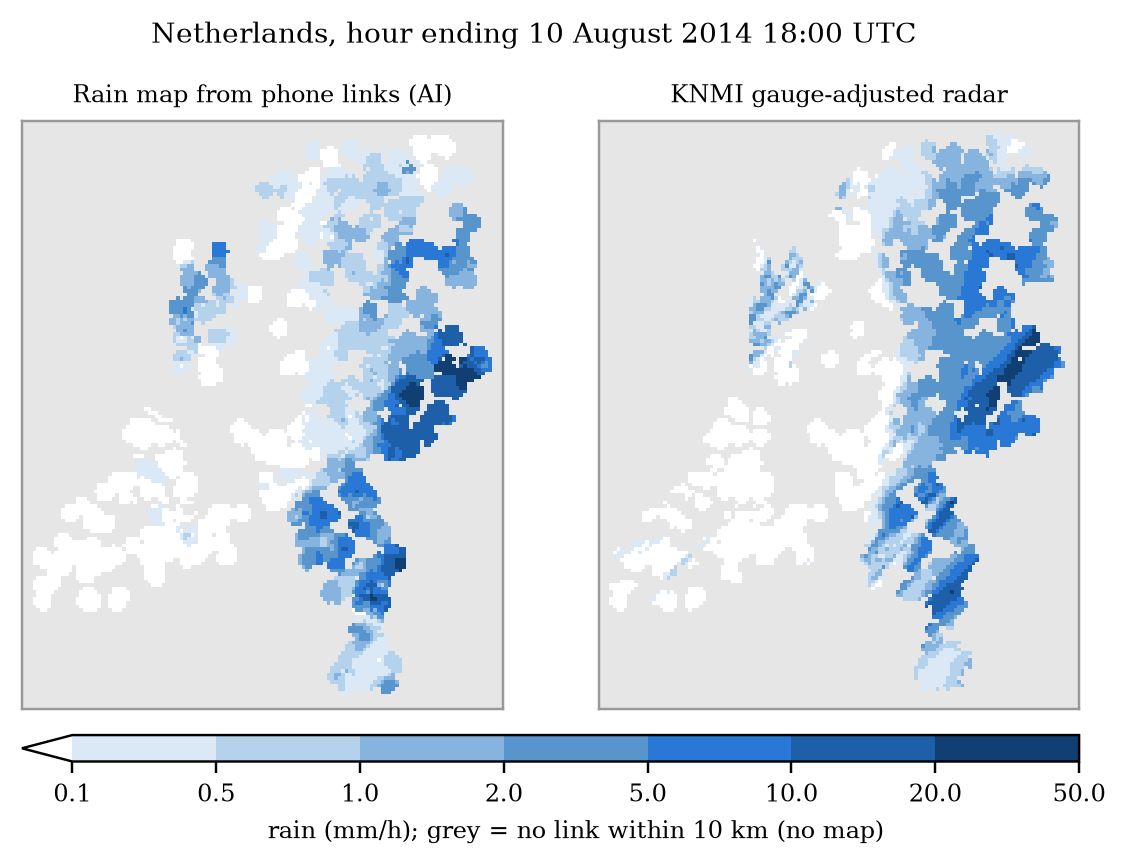
\includegraphics[width=0.82\textwidth]{fig_nl_map.png}
\caption{The wettest hour of the Dutch summer in our data. Left: rain map made only from phone links (AI, 1{,}653 sub-links).
Right: KNMI's gauge-adjusted radar for the same hour and the same squares. The link map gets the big picture right: the
band of rain from south to north-east, dry in the west, the heaviest cores in the east. It is blotchier (each link makes a
round patch around itself) and misses the finest detail.}
\label{fig:nl_map}
\end{figure}

\begin{oneline}
Where links are dense, a map made from them matches rain gauges better than a weather radar does; the map stays useful up to
about 5\,km from the nearest link and is blank beyond 10\,km.
\end{oneline}

%==========================================================
\section{Forecasting the next hour}
\label{sec:nowcast}
%==========================================================

A flood warning is most useful before the rain arrives. The simplest forecast of the next hour, called
\textbf{nowcasting}, does not need any weather physics: watch how the rain pattern moved over the last half hour and assume
it keeps moving the same way.

\subsection{How it works}
\begin{enumerate}
\item \textbf{Find the motion.} Take the last three maps (30 and 15 minutes ago, and now). For each part of the map, look
for the shift that best lines up the earlier pattern with the later one. This is called \textbf{optical flow}; it is the
same idea a phone camera uses to steady a shaky video. We used the Lucas--Kanade method from \textbf{pysteps}, a free
nowcasting toolkit used by weather services.
\item \textbf{Move the map.} Push every square of the current map along its arrow, 15 minutes at a time, up to 60 minutes
(\emph{semi-Lagrangian extrapolation}: each square of the forecast looks back along the arrows to find where its rain is
coming from).
\item \textbf{Compare with a lazy forecast.} \textbf{Persistence} assumes the rain stays exactly where it is now. A
nowcast is only worth something if it beats that.
\end{enumerate}

\subsection{Scoring a forecast: the critical success index}
Pick a threshold, say 1\,mm/h. Over all squares, count \textbf{hits} (forecast and observed both above it), \textbf{misses}
(observed above, forecast below) and \textbf{false alarms} (forecast above, observed below). Then
\[
\text{CSI} = \frac{\text{hits}}{\text{hits} + \text{misses} + \text{false alarms}} .
\]
1 is perfect; 0 means the forecast never put rain in the right place. Squares where both say ``dry'' do not count, so a
forecast cannot score well just by saying ``dry'' over a mostly dry country.

\begin{example}[: CSI]
On one map, 300 squares are forecast wet and 400 are observed wet; 200 of them overlap. Hits 200, misses
$400-200 = 200$, false alarms $300-200 = 100$. CSI $= 200 / (200+200+100) = 0.40$.
\end{example}

\subsection{Results}
We made a nowcast at every full hour of the Dutch summer when rain covered at least 800\,km$^2$ of the network: 612 hours.
\begin{center}
\begin{tikzpicture}
\begin{axis}[width=0.62\textwidth,height=5cm,xmin=10,xmax=65,ymin=0,ymax=0.5,xtick={15,30,45,60},
  xlabel={forecast lead time (minutes)},ylabel={CSI at 1 mm/h},grid=major,grid style={inkc!12},
  tick label style={font=\small},label style={font=\small},
  legend style={font=\scriptsize,draw=none,fill=white,fill opacity=0.85,text opacity=1},legend cell align=left,legend pos=north east]
  \addplot[thick,color=inkc,mark=*,mark size=1.6pt] table[x=lead,y=nowcast] {nowcast_csi.dat};
  \addlegendentry{nowcast (moving the map)}
  \addplot[thick,dashed,color=gaugec,mark=square*,mark size=1.4pt] table[x=lead,y=persistence] {nowcast_csi.dat};
  \addlegendentry{persistence (rain stays put)}
\end{axis}
\end{tikzpicture}
\end{center}
\begin{center}\small
\begin{tabular}{lcccc}
\toprule
Lead time & 15 min & 30 min & 45 min & 60 min\\
\midrule
CSI at 1\,mm/h, nowcast & \textbf{0.45} & \textbf{0.28} & \textbf{0.20} & \textbf{0.16}\\
CSI at 1\,mm/h, persistence & 0.44 & 0.27 & 0.19 & 0.15\\
\bottomrule
\end{tabular}
\end{center}
These scores compare the forecast with the link map that was actually observed later. As an independent check we also
compared the forecast rain for the whole next hour with KNMI's radar for that hour: CSI 0.26 for the nowcast against 0.24
for persistence, correlation 0.30 against 0.26.

\begin{figure}[h]
\centering
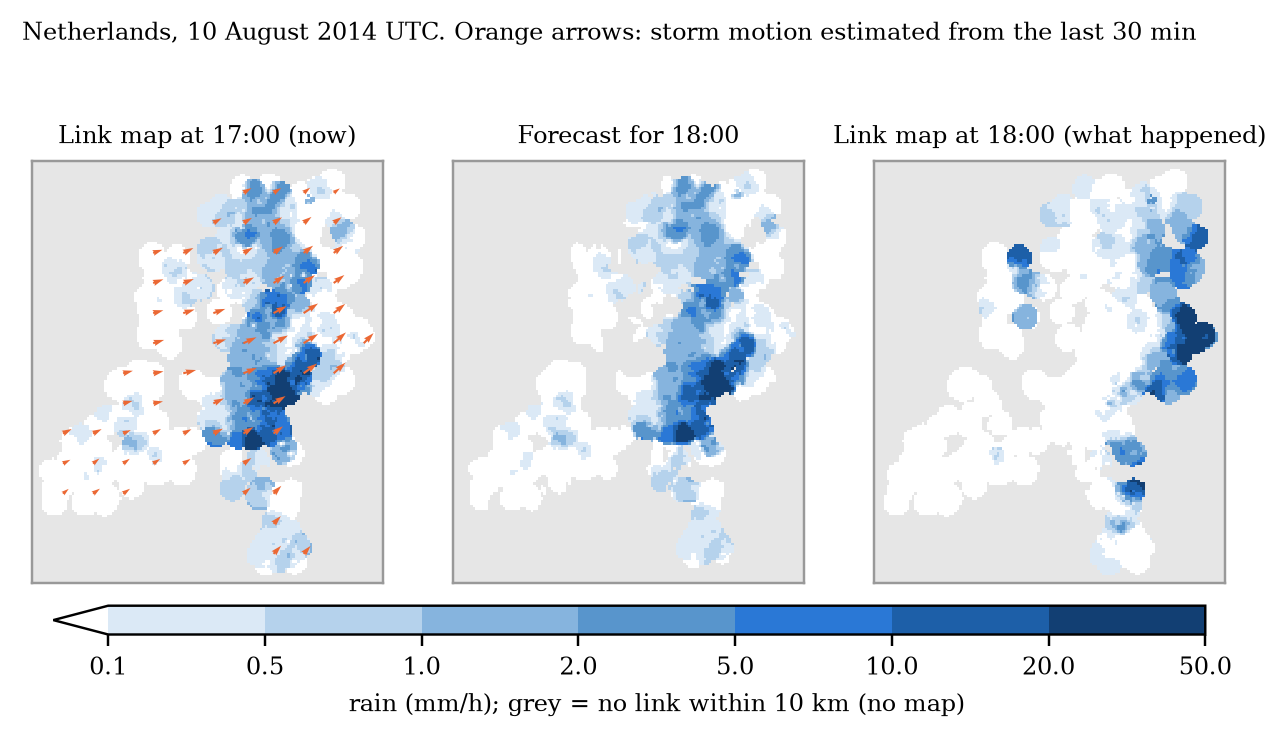
\includegraphics[width=0.95\textwidth]{fig_nowcast.png}
\caption{A nowcast during the same storm as Figure~\ref{fig:nl_map}. Left: the link map at 17:00 and the motion found from the
last 30 minutes (towards the north-east). Middle: that map moved forward 60 minutes. Right: what the links actually saw at
18:00. The direction was right, but the storm moved faster than forecast and by 18:00 its heaviest part was already
leaving the network on the east side.}
\label{fig:nowcast}
\end{figure}

\textbf{Honest reading.} The nowcast beats persistence at every lead time and in both checks, but only by a little. Skill
falls quickly: after 30 minutes, fewer than a third of the 1\,mm/h areas are in the right place. Three reasons, all visible
in Figure~\ref{fig:nowcast}:
\begin{itemize}
\item \textbf{Blotchy maps.} Each link makes a round patch on the map, and patches flicker as links switch between ``wet''
and ``dry''. Optical flow then partly tracks the flicker instead of the storm.
\item \textbf{Blind edges.} Rain that is about to enter the network from outside is invisible until it arrives, and rain
leaving it disappears. Radar sees 100+\,km beyond any city.
\item \textbf{Coarse steps.} The Dutch data come every 15 minutes; radar nowcasting usually uses 5-minute images.
\end{itemize}

\begin{oneline}
Moving the link map along the storm's motion gives a forecast that beats ``rain stays put'' up to an hour ahead, but only
slightly; for useful 30--60 minute warnings the motion should come from a wider view (radar or satellite), with the links
providing the accurate rain inside the city.
\end{oneline}

%==========================================================
\section{What Phase 3 taught us}
\label{sec:phase3_end}
%==========================================================

\begin{itemize}
\item \textbf{Maps from links work where links are.} In Gothenburg, link maps match rain gauges better than the weather
radar (correlation 0.92 and 0.89 against 0.80). In Italy and the Netherlands the AI maps are good within about 5\,km of a
link and far better than the classical ones.
\item \textbf{Coverage follows people.} Away from towns there are no links and no map: 145 of 319 Italian gauges are more
than 10\,km from any link. For Algeria this means link maps for cities and valleys with towers, and something else (radar
where it exists, satellites) everywhere else.
\item \textbf{Forecasting from links alone is weak.} The nowcast beats persistence, but by a small margin.
\end{itemize}

\textbf{Next:}
\begin{enumerate}
\item Better nowcasts by taking the storm motion from a wider view: satellite rain (NASA's IMERG, every 30 minutes,
worldwide), and radar where available, while keeping the links' accurate rain inside the city.
\item Phase~4: a simulated Algerian network on real tower positions, fed with real storms, to show the whole chain working
on Algeria (clearly labelled as a simulation).
\end{enumerate}


%==========================================================
\appendix
\section{Glossary}
%==========================================================
\small
\begin{description}[leftmargin=3.2cm,style=nextline,itemsep=0.25em]
\item[Attenuation] Weakening of a signal, measured in dB.
\item[Backhaul] The part of a phone network that connects towers to each other and to the core network.
\item[Baseline] The normal, dry-weather level of a link's total loss.
\item[dB (decibel)] Ten times the base-10 logarithm of a power ratio. $+3$\,dB $\approx$ double, $-10$\,dB = one tenth.
\item[dBm] Power compared with 1 milliwatt, in decibels. 0\,dBm = 1\,mW.
\item[Electromagnetic wave] A travelling pattern of electric and magnetic fields. Light and radio are both examples.
\item[Free-space path loss] The weakening of a beam caused only by spreading out over distance.
\item[Frequency] Number of wiggles per second, in hertz (Hz). 1\,GHz = one billion per second.
\item[Fresnel zone] The cigar-shaped region around the straight line between two dishes where the radio energy travels.
\item[Gain (antenna)] How much a dish concentrates power in its pointing direction, in dB.
\item[ITU-R P.838] The international standard that gives the $a$ and $b$ coefficients linking rain rate and loss.
\item[Line of sight] A clear straight path between two antennas.
\item[MCC] Matthews correlation coefficient. A score for yes/no detection; 1 is perfect, 0 is random.
\item[Microwave link] A pair of dish antennas exchanging a radio beam between two towers.
\item[mm/h] Millimetres of rain per hour: the depth of water a rain intensity would leave after one hour.
\item[Multipath fading] Signal dips when parts of the beam take slightly different paths and partly cancel.
\item[Polarisation] The direction in which the wave's electric field wiggles: vertical or horizontal.
\item[Quantisation] Rounding of the recorded signal to fixed steps (e.g.\ 0.1\,dB or 1\,dB).
\item[Radome] The protective plastic or fabric cover over a dish antenna.
\item[RMSE] Root mean square error: the typical size of a mistake, with large mistakes weighted more.
\item[RSL] Received signal level: power arriving at the receiving dish, in dBm.
\item[Specific attenuation $k$] Loss per kilometre of rainy path, in dB/km.
\item[Standard deviation] How far values typically stray from their average; used here to measure how jumpy a signal is.
\item[Sub-link] One direction of a two-way link.
\item[TSL] Transmitted signal level: power sent by the transmitting dish, in dBm.
\item[Wavelength] Distance between two wave crests. Equals the speed of light divided by the frequency.
\item[Wet antenna attenuation] Extra loss caused by a film of water on the radome, not by rain along the path.
\end{description}
\normalsize

\section{Sources}
\small
\begin{itemize}
\item ITU-R Recommendation P.838-3 (2005), \emph{Specific attenuation model for rain for use in prediction methods}. International Telecommunication Union.
\item H. Messer, A. Zinevich, P. Alpert (2006), \emph{Environmental monitoring by wireless communication networks}, Science 312, 713. The first paper to propose this idea.
\item A. Overeem, H. Leijnse, R. Uijlenhoet (2013), \emph{Country-wide rainfall maps from cellular communication networks}, PNAS 110, 2741--2745. Rain maps for the whole Netherlands from phone links.
\item M. Schleiss, A. Berne (2010), \emph{Identification of dry and rainy periods using telecommunication microwave links}, IEEE Geoscience and Remote Sensing Letters 7, 611--615. The ``jumpy signal'' wet/dry method of Step~2.
\item J. Andersson et al. (2022), \emph{OpenMRG: Open data from Microwave links, Radar, and Gauges for rainfall quantification in Gothenburg, Sweden}, Earth System Science Data 14, 5411--5426. Dataset: doi:10.5281/zenodo.7107689 (CC BY-SA 4.0).
\item pycomlink, open-source Python library for microwave-link rain retrieval (version 0.6.0), \url{https://github.com/pycomlink/pycomlink}. Source of the ITU coefficients and the wet-antenna model used here.
\end{itemize}
All project results quoted here are in \texttt{results/phase1\_openmrg.md} of the project repository.


%==========================================================
% Appendix additions for Part 2
%==========================================================
\section{More words, from Parts 2 and 3}
\small
\begin{description}[leftmargin=3.2cm,style=nextline,itemsep=0.25em]
\item[Ablation] Removing one ingredient of a method to see how much it was helping.
\item[Ascend] Huawei's family of chips designed for AI calculations.
\item[Augmentation] Showing training examples in slightly altered forms (here: rounded to whole decibels) so the network does not depend on details that change between networks.
\item[Bias (of a neuron)] A fixed number a neuron adds to its weighted sum. Not the same as the \emph{bias} score of Section~\ref{sec:scores}.
\item[Causal] Using only the present and the past, never the future. Needed for live warnings.
\item[CSI] Critical success index: hits divided by (hits + misses + false alarms) for rain above a threshold. 1 is perfect.
\item[Convolution] A small set of weights that slides along the signal, producing one new number per position.
\item[Cross-validation] Judging every part of the data in turn with a model trained on all the other parts, so everything gets an honest test.
\item[Dry level] What a link's total loss would be if it were dry right now. Ours: the 20th percentile of the previous 3 days.
\item[Dilation] Spacing the minutes a convolution looks at further apart (1, 2, 4, \ldots), so a few layers can see far back.
\item[GPU] Graphics card: a chip that performs many multiplications at once, which makes training fast.
\item[Gauge-adjusted radar] Radar rain maps corrected with many rain gauges; a better reference than radar alone.
\item[Loss (penalty)] In AI, one number measuring how wrong the network's answers were. Not the signal loss in dB.
\item[IDW] Inverse-distance weighting: a map square takes a weighted average of nearby links, closer links counting more ($1/d^2$).
\item[Kriging] A cleverer way to make maps that learns from the data how quickly rain changes with distance.
\item[Median] The middle value of a sorted list. Barely moved by a few extreme values.
\item[Min/max data] Only the weakest and strongest received level of every 15 minutes, as many operators store.
\item[MindSpore] Huawei's free toolkit for building and training neural networks.
\item[ModelArts] Huawei Cloud's service for training and running AI models.
\item[Nowcasting] Forecasting the next minutes to hours by moving the current rain map along its recent motion.
\item[Neighbour check] Counting a link's rain only if another link within 10\,km also reports rain within 15 minutes.
\item[Neural network] A large adjustable formula made of layers of simple calculators (neurons), whose dials are set by learning from examples.
\item[Percentile] The value a given share of the way up a sorted list. The 20th percentile has 20\% of the values below it; the median is the 50th.
\item[Optical flow] Finding how a pattern moved between two images.
\item[Overfitting] Doing well on the training examples but badly on new ones: memorising instead of learning.
\item[Persistence] The lazy forecast: rain stays exactly where it is now. A nowcast must beat it.
\item[Pooled score] A score computed over all links and hours mixed together. Sensitive to a few wild values.
\item[pysteps] A free nowcasting toolkit used by weather services; we use its optical flow and extrapolation.
\item[PyTorch] A widely used free toolkit for neural networks; our local default.
\item[RAINLINK] The min/max rain retrieval algorithm developed for the Dutch link data.
\item[Reliability score] Our test of whether to trust a link: does its signal drop alone (unconfirmed by its 5 nearest neighbours) or all the time (more than 20\% of the time)?
\item[Receptive field] How far into the past the network's answer can depend on: 1{,}021 minutes for ours.
\item[Strength (of a run)] The AI's rain divided by the reference's, at the moments when both say it rains. 1.00 is perfect.
\item[Signal event] A quarter-hour in which a link's loss is at least 1.5\,dB above its own dry level.
\item[Seed] The starting point of the random numbers used in training. Different seeds give slightly different networks.
\item[Sigmoid] The function $1/(1+e^{-x})$, which turns any number into a probability between 0 and 1.
\item[TCN] Temporal convolutional network: a network of stacked, dilated, causal convolutions along time.
\item[Threshold] The probability above which we say ``raining''. Ours is 0.25, chosen on the validation data.
\item[Training / validation / test] The three separate piles of data: to learn from, to choose with, to judge once.
\item[Weight] One of the network's adjustable numbers (a dial), multiplying one input of a neuron.
\item[Zero-shot] Using a model on a place or kind of data it never learned from, with no changes.
\end{description}
\normalsize

\section{Sources for Parts 2 and 3}
\small
\begin{itemize}
\item S. Bai, J. Z. Kolter, V. Koltun (2018), \emph{An empirical evaluation of generic convolutional and recurrent networks for sequence modeling}, arXiv:1803.01271. The temporal convolutional network design.
\item J. Polz, C. Chwala, M. Graf, H. Kunstmann (2020), \emph{Rain event detection in commercial microwave link attenuation data using convolutional neural networks}, Atmospheric Measurement Techniques 13, 3835--3853. Earlier work showing neural networks can detect rain in link data.
\item A. Overeem, H. Leijnse, R. Uijlenhoet (2016), \emph{Retrieval algorithm for rainfall mapping from microwave links in a cellular communication network}, Atmospheric Measurement Techniques 9, 2425--2444. The RAINLINK method.
\item E. Covi, G. Roversi, R. Nebuloni (2026), \emph{OpenRainER: an open-source dataset for studying the opportunistic sensing of rainfall in Emilia-Romagna, Italy}, Earth System Science Data Discussions, doi:10.5194/essd-2026-160. Dataset: doi:10.5281/zenodo.10593848 (CC BY 4.0, version 2.0.3).
\item A. Overeem et al., \emph{Four-year commercial microwave link dataset for the Netherlands}, 4TU.ResearchData, \url{https://doi.org/10.4121/be252844-b672-471e-8d69-27269a862ec1} (CC BY 4.0). We used June--August 2014.
\item KNMI, \emph{Precipitation -- climatological gauge-adjusted radar hourly accumulations for the Netherlands (RAD\_NL25\_RAC\_MFBS\_01H)}, KNMI Data Platform, version 2.0.
\item S. Pulkkinen et al. (2019), \emph{Pysteps: an open-source Python library for probabilistic precipitation nowcasting (v1.0)}, Geoscientific Model Development 12, 4185--4219. The nowcasting toolkit of Part~3 (we used version 1.21).
\item MindSpore, Huawei's open-source deep-learning framework, version 2.10, \url{https://www.mindspore.cn}. PyTorch version 2.11, \url{https://pytorch.org}.
\end{itemize}
All Part~2 numbers are in \texttt{results/phase2.md} and \texttt{results/phase2\_summary.json}; Part~3 numbers in \texttt{results/phase3\_maps.json} and \texttt{results/phase3\_nowcast.json} of the project repository.
\normalsize

\end{document}
